% This section reworked to have all the major PD subsystems as sections. 

%%%%%%%%%%%%%%%%%%%%%%%%%%%%%%%%%%%%%%%%%%%%%%%%%%%%%%%%%%%%%%%
%\section{Photon Detection System Design}

%%%%%%%%%%%%%%%%%%%%%%%%%%%%%%%%%%%
\section{Light Collectors}
\label{sec:fdsp-pd-lc}

The \dword{xarapu}, adopted as the baseline design, is an evolution of the \dword{arapuca} concept that further improves the collection efficiency, while retaining the same working principle, mechanical form factor and active photosensitive coverage. 
 In the original \dword{arapuca} concept, two wavelength-shifters were coated on either side of the dichroic filter window. 
 In contrast, the \dword{xarapu} replaces the inner surface coating with a wavelength-shifter-doped %polyvinyl toluene (PVT) 
 polystyrene light guide\footnote{Eljen EJ-286\texttrademark{}.} occupying a portion of the cell volume, with the silicon photosensor readout mounted along the narrow sides of the cell, as illustrated in Figure~\ref{fig:pds-x-arapuca-cell}. The model shown is a single cell design used for prototypes that allows for photons to enter from either face, however one window can be replaced with an opaque reflecting surface for sensitivity through just one face.

Photons entering the light guide plate are absorbed and wavelength-shifted with high efficiency, and some fraction (those incident on the plate surface at greater than the critical angle) are transported to the readout via total internal reflection. The \dword{lar} gaps between the plate and the surfaces of the cavity ensure the discontinuity of the refractive index that contributes to effective trapping of the photons (n$_{plate}$=1.58 and n$_{LAr}$=1.24 for the wavelengths emitted by the plate).
Those exiting the plate reflect off the filter or other highly reflecting surfaces of the cell, with some fraction eventually incident on a \dword{sipm}, as in a standard \dword{arapuca} cell.
\dword{xarapu} is thus effectively a hybrid solution between the \dword{sarapu} and the \dword{wls} light guide concepts implemented in \dword{pdsp}.



This solution minimizes the number of reflections on the internal surfaces of the cell and thus minimizes the probability of photon loss. 
We have performed a full numerical description of the \dword{xarapu} using the Geant4 framework, following previous studies done for the \dword{sarapu} device~\cite{Marinho:2018doi}.  The comparison between the two kinds of devices is dependent on the value of absorption length of the bar, which was not known precisely, so the gain in efficiency for the \dword{xarapu} with the dimensions tested at \dword{unicamp} is estimated to be between 15 and 40\% when compared to the \dword{sarapu} with same dimensions and number of \dwords{sipm}.
Results from prototype measurements are presented in Sections~\ref{sec:xarapuca-unicamp} and \ref{sec:iceberg-teststand} and are consistent with the simulations.

 \begin{dunefigure}[\dshort{xarapu} conceptual model]{fig:pds-x-arapuca-cell}
{Simplified conceptual model depicting a \dword{xarapu} cell design sensitive to light from both sides: assembled cell (left),  exploded view (right). The yellow plates represent the dichroic filters (coated on their outside surfaces with \dword{ptp} \dword{wls}), the pale blue plate represents the wavelength shifting plate, and the photosensors are visible on the right side of the cell. The size and aspect ratio of the cells can be adjusted to match the spatial granularity required for a \dword{pd} module. .
} 
 % \vspace{-2.5cm}
 %two-sided x-arapuca 4/14/18 
  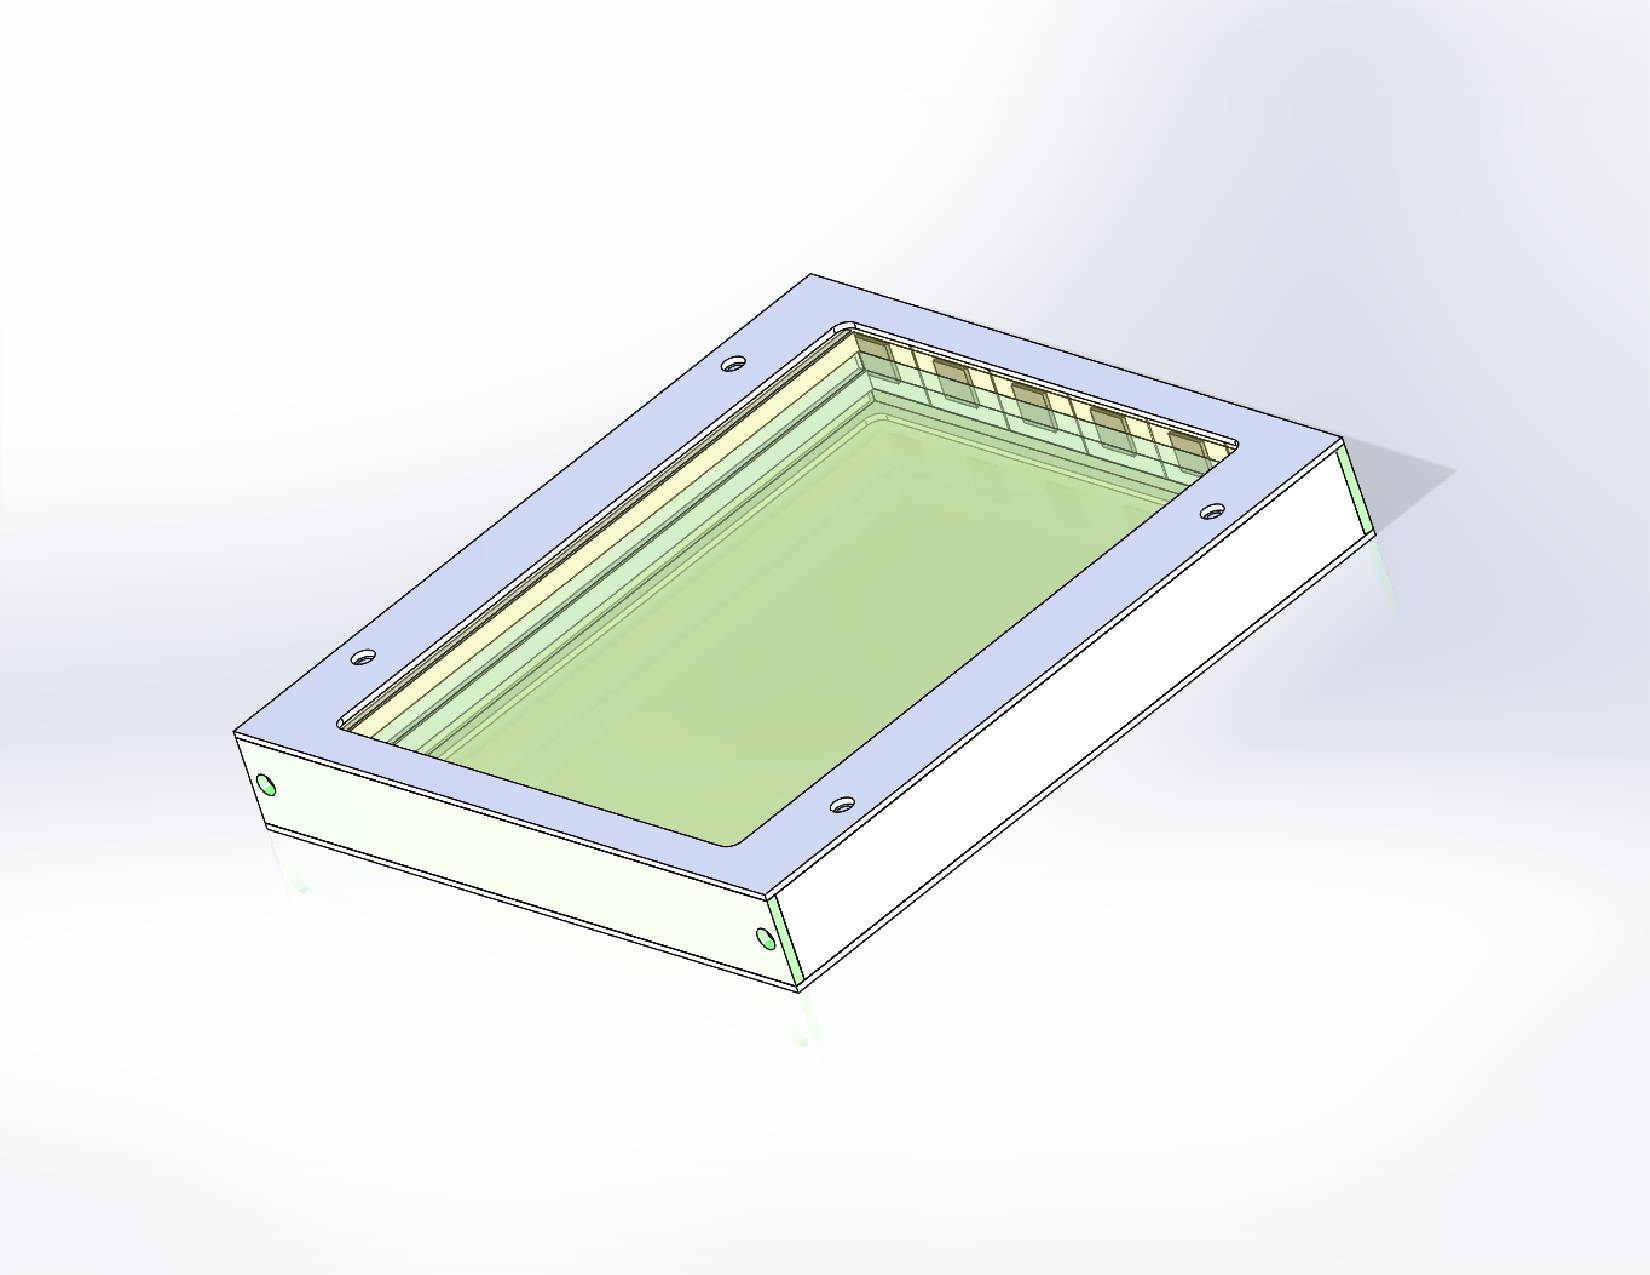
\includegraphics[height=.25\textheight]{graphics/pds-x-arapuca-cell}
  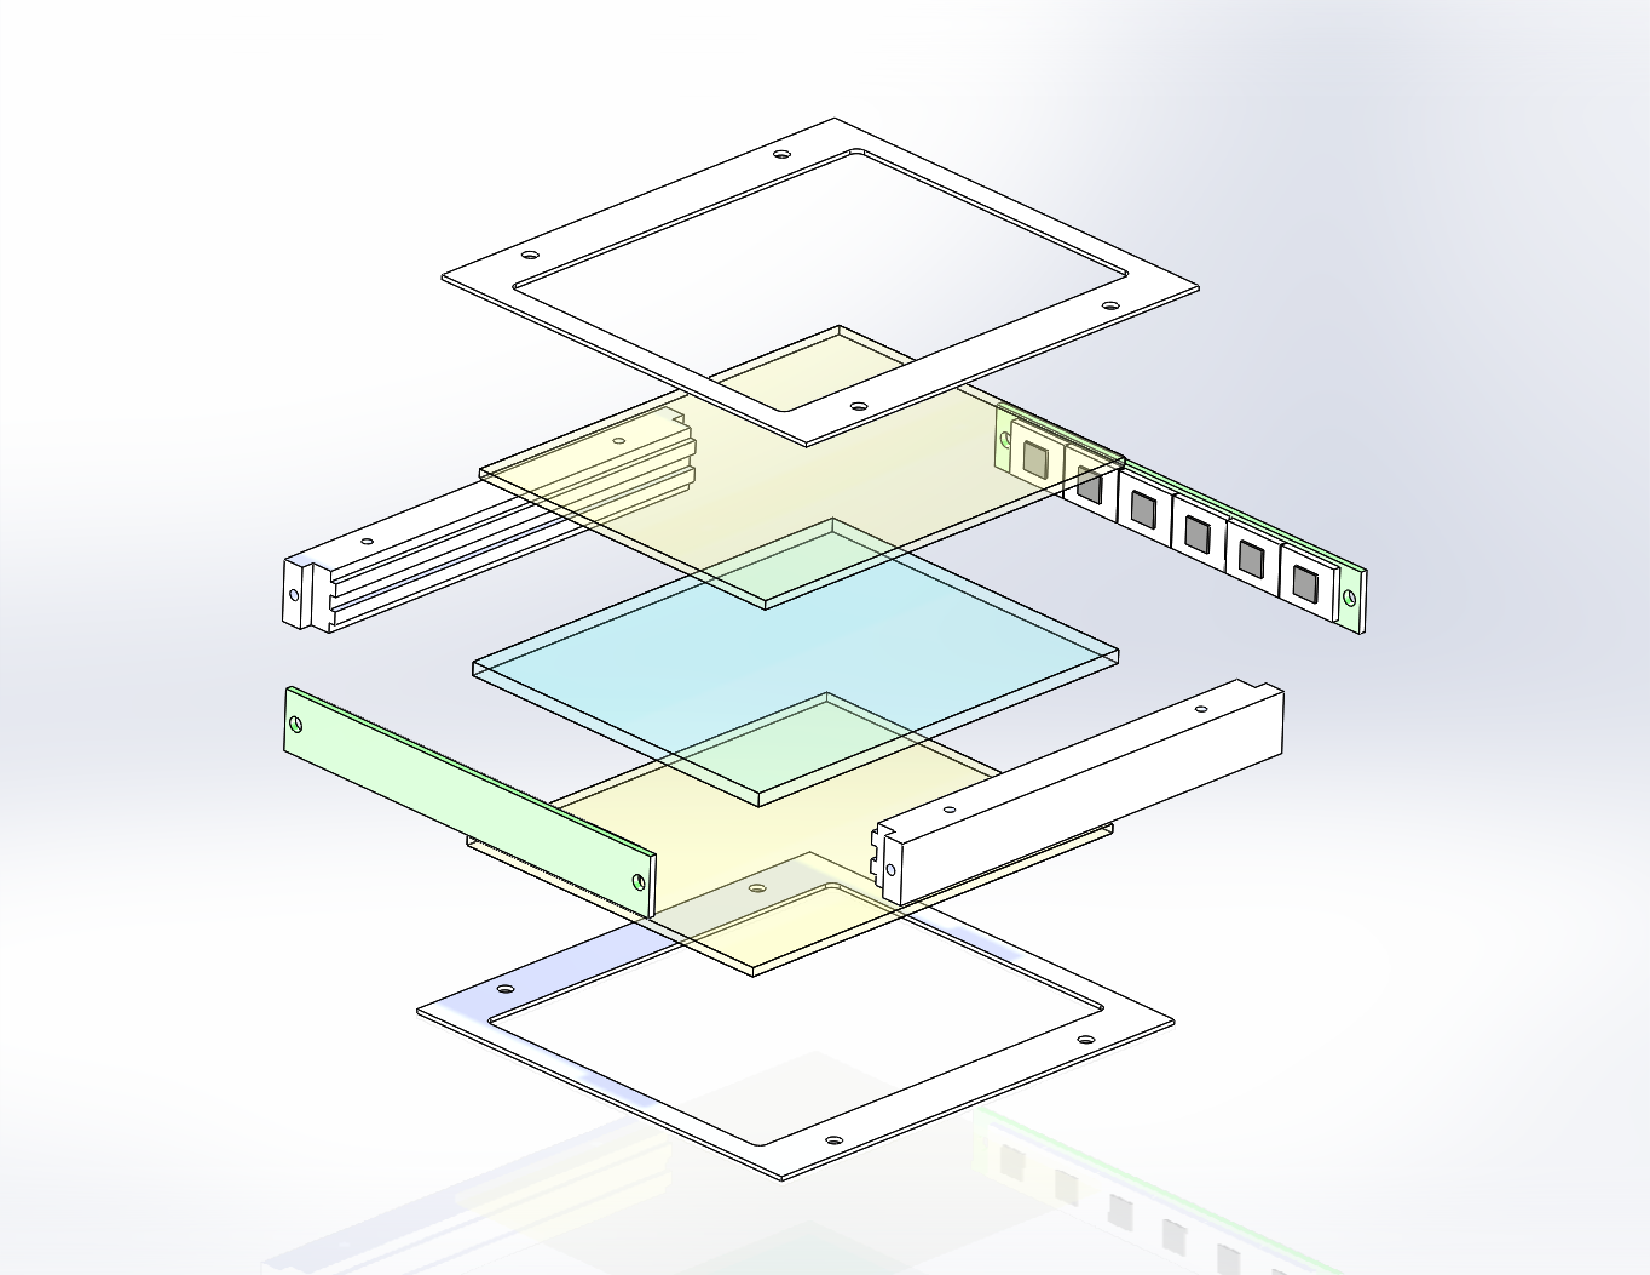
\includegraphics[height=.25\textheight]{graphics/pds-x-arapuca-exploded-view}
\end{dunefigure}

The  \dword{pd} module designed for the \dword{dune} \dword{spmod}, illustrated in Figure~\ref{fig:pds-x-arapuca-full-module}, consists of four supercells, each containing a rectangular 
light guide inside the cell positioned behind an array of six dichroic filters that form the entrance window.  
This design is easily configurable to detect light from just one side, as required for the side \dword{apa}s, or from both sides for the central \dword{apa}s. 

For dual-sided \dword{xarapu} modules, dichroic filters are placed on both sides of the cell facing the drift volumes.  In the case of the single-sided device, the back side of the cell has a layer of highly reflective Vikuiti\footnote{3M Vikuiti\texttrademark\  ESR - http://multimedia.3m.com/mws/media/193294O/vikuiti-tm-esr-application-guidelines.pdf} to act as a  reflector.  In both cases, the \dword{sipm} arrays are installed on two of the narrow sides of the cell perpendicular to the windows, parallel to and up against the light guide thin ends. Half of the \dword{sipm} active detection area collects photons from the light guide, a quarter of the area on either side of the guide is free to collect the fraction of photons reflected off the cell walls and windows. 
This fraction of photosensor coverage for photons emerging from the light guide ends is a result of using a standard \num{6}$\times$\SI{6}{mm$^2$} \dword{sipm} placed symmetrically with respect to the mid-plane of the bar. Simulation of two additional \dword{sipm} geometries with the same active area (\num{4}$\times$\SI{9}{mm$^2$} and \num{3}$\times$\SI{12}{mm$^2$}) showed no substantial difference in the detection efficiency that would justify a custom geometry for the \dword{sipm}.

The basic mechanical design of the \dword{xarapu}-based \dword{pd} modules is similar to that of the two prototypes produced for \dword{pdsp}. 
The prototype design was modified to include mechanical changes to allow both single-sided and dual-sided readout; an increase in the light collection area made possible by larger slots in the \dword{apa}; and a modified cabling and connector plan necessary to move the \dword{pd} cables out of the \dword{apa} side tubes while reducing cable requirements to one Cat-6 cable per \dword{pd} module.

\begin{dunefigure}[\dshort{xarapu} module indicating four supercells]
{fig:pds-x-arapuca-full-module}
{\dword{xarapu} module overview. A module, which spans the width of an \dword{apa}, includes 24
 \dword{xarapu} cells, grouped into a set of four supercells of six cells each. In the center, active ganging \dwords{pcb} collect the signals and mechanically connect the supercells.}
   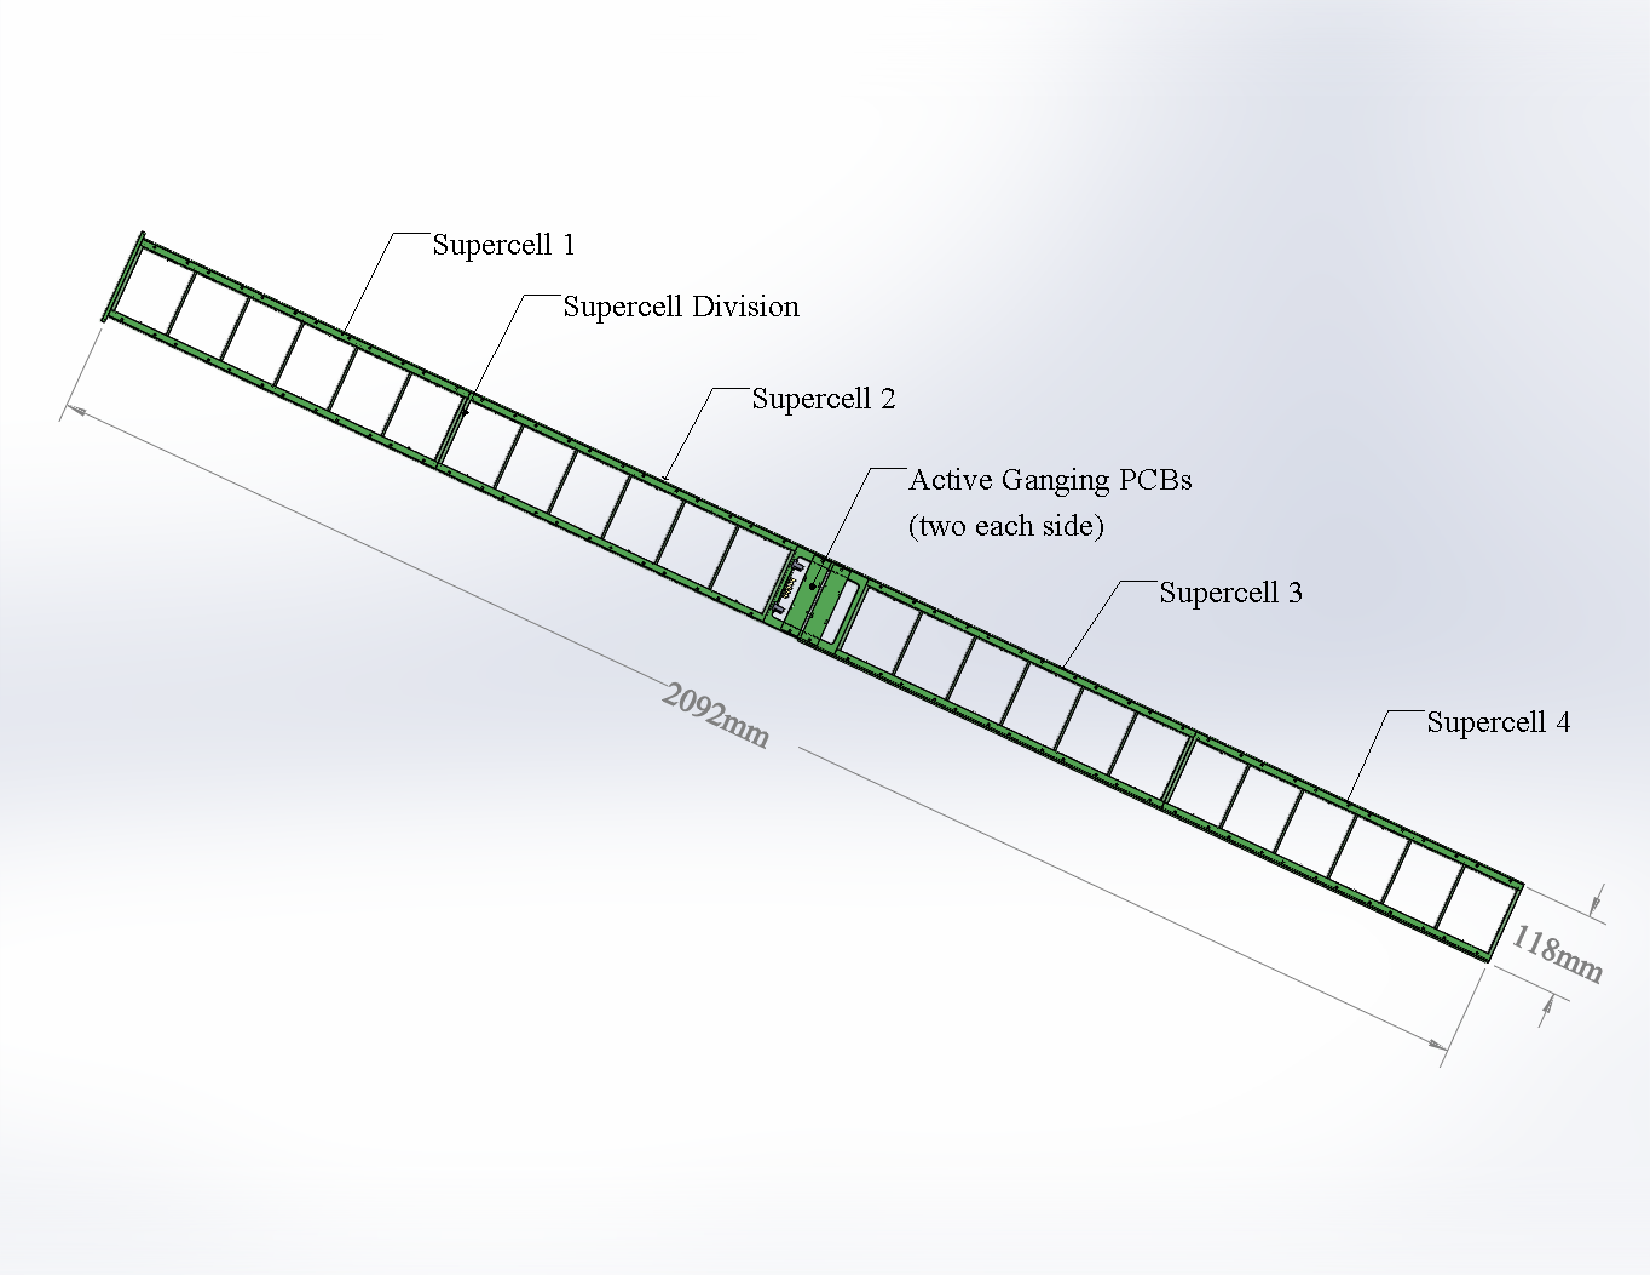
\includegraphics[width=17cm]{graphics/pds-design-full-module-dimensioned-2}
\end{dunefigure}

An \dword{xarapu} module is assembled in a bar-like configuration with external dimensions inside the \dword{apa} frame of \SI{2092}{mm}$\times$\SI{118}{mm}$\times$\SI{23}{mm},  allowing insertion between the wire planes through each of the ten slots (five on each side) in an \dword{apa}. In addition, there is a header block \SI{5}{mm}(long)$\times$\SI{135}{mm}(wide) at the insertion side of the module used to fix the module inside the \dword{apa} frame, bringing the maximum length to \SI{2097}{mm} and the maximum width to \SI{135}{mm}.
The module contains four \dword{xarapu} supercells, each with six dichroic filter-based optical windows (for the single-sided readout) or twelve windows (double-sided readout) with an exposed area of \SI{78}{mm}$\times$\SI{93}{mm}.  
The total window area for each (single-sided) supercell \dword{xarapu} is \SI{43524}{mm$^2$}.
The internal dimensions of a supercell are approximately \SI{488}{mm}$\times$\SI{100}{mm}$\times$\SI{8}{mm}. A \dword{wls} plate (Eljen EJ-286) of dimensions \SI{487}{mm}$\times$\SI{93}{mm}$\times$\SI{3.5}{mm} is centered in the supercell midway between the dichroic windows. 

The thickness of \SI{3.5}{mm} for the plate is chosen to allow the almost complete absorption of the photons wavelength-shifted by the \dword{ptp} and to ensure the nominal conversion efficiency. This thickness allows a \SI{2}{mm} \dword{lar} gap on both sides of the plate, which prevents any physical contact of the surfaces even considering the tolerances on material thicknesses and plate flatness.   

\begin{dunefigure}[Exploded \dshort{xarapu} supercell]{fig:pds-x-arapuca-exploded-Detail}
{Detailed exploded view of \dword{xarapu} supercell. Note that components are designed to be cut from \frfour G-10 sheets to simplify fabrication.}
 %two-sided x-arapuca 4/14/18
   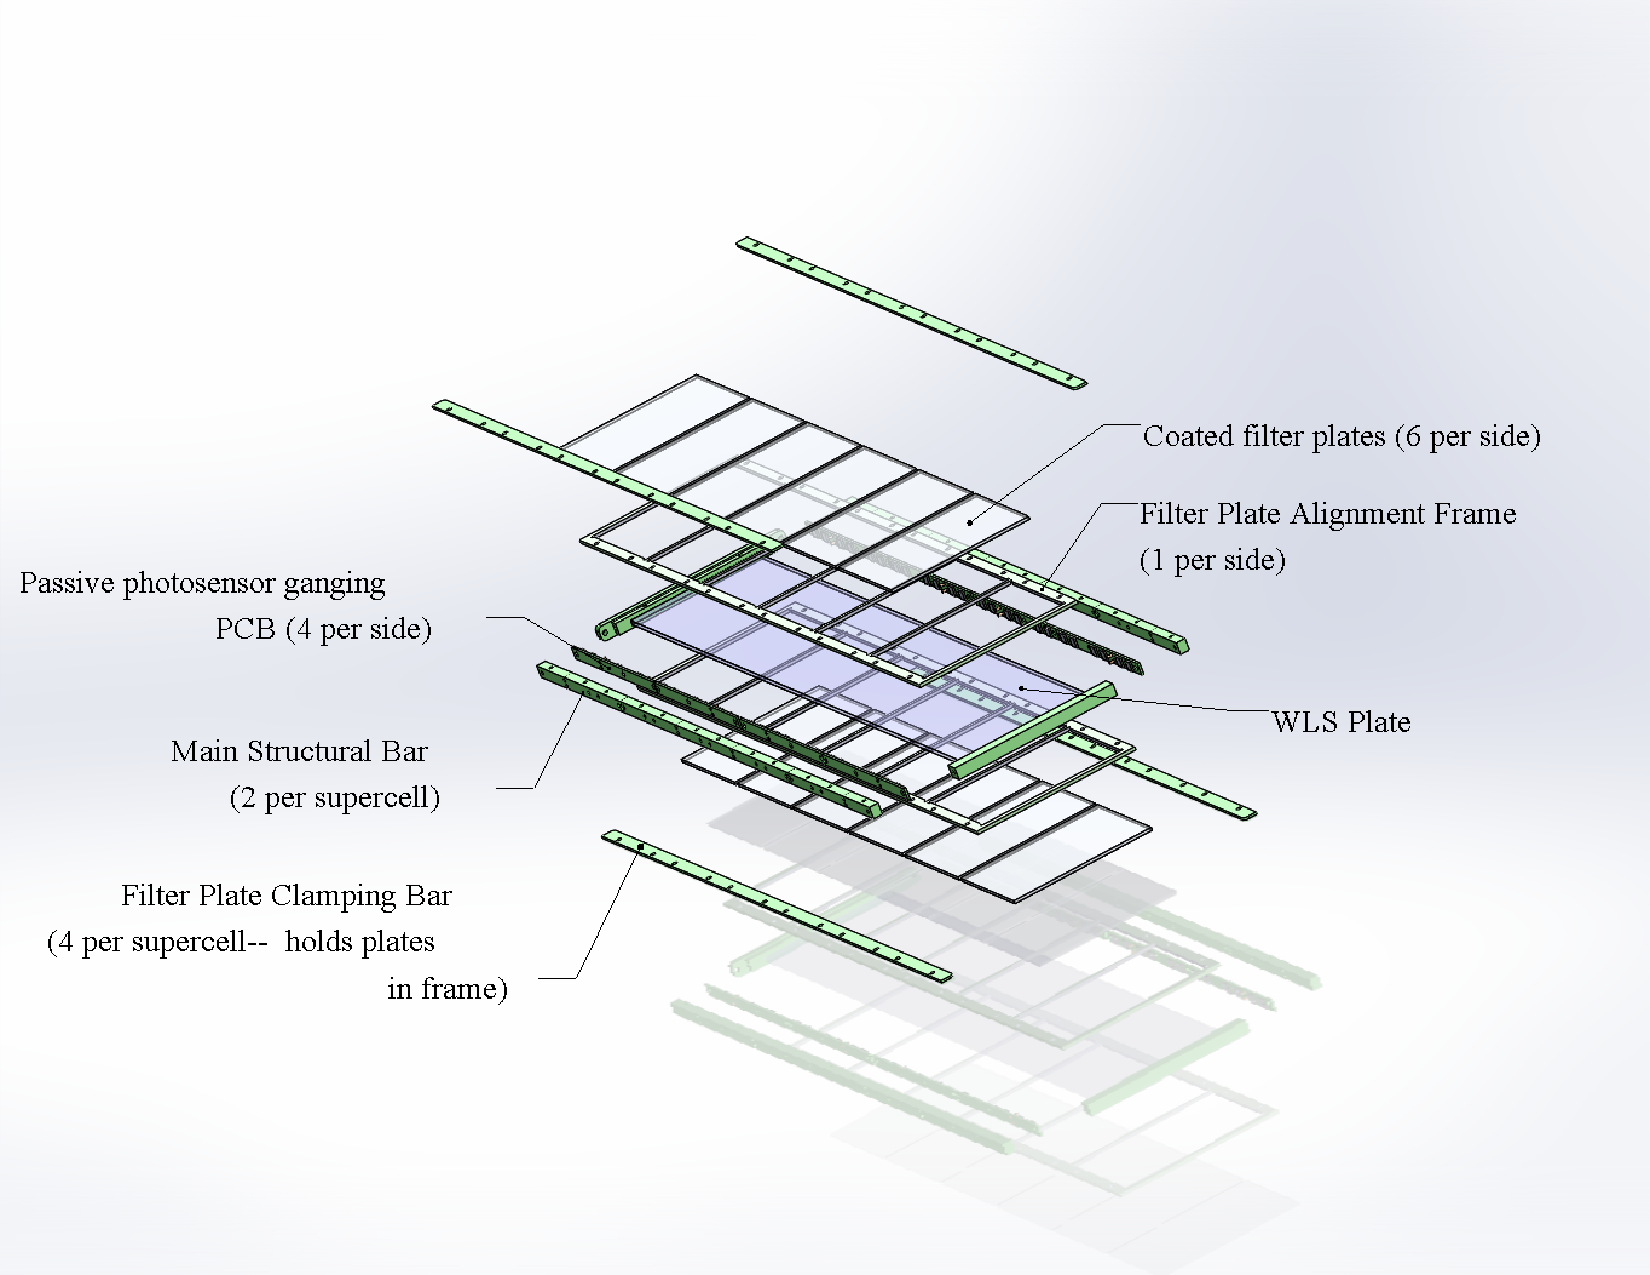
\includegraphics[height=.55\textheight]{graphics/pds-exploded-supercell-assembly-r3}
\end{dunefigure}

To reduce production costs and simplify fabrication, most of the \dword{pd} components are designed to be water-jet cut from sheets of \frfour G-10 material, with minimal post-cutting machining required (mostly the tapping of pre-cut holes).  The current design contains many small fasteners; we will investigate replacing some of the fasteners with epoxy lamination of cut sheets where appropriate and cost effective.


The \dwords{sipm} are mounted to \dwords{pcb} called ``photosensor mounting boards'' that  are positioned on the long sides of the supercell.  
Six \dwords{sipm} are mounted to a single photosensor mounting board.  The mounting boards incorporate spacers that position the face of the photosensors a nominal \SI{0.5}{mm} from the face of the \dword{wls} plate.  All six are electrically connected in parallel (``passively ganged'').

 Before mounting the boards into the \dword{xarapu} module, the boards are tested at room and \dword{ln} temperatures. 
 Each supercell uses eight photosensor mounting boards, each with six \dwords{sipm} (Figure~\ref{fig:mounting-board-routing-board}~(top)), 
 to accommodate the 48 \dwords{sipm}.  The ganged signal outputs from these boards are connected to traces in signal routing boards at the edge of the \dword{pd} module. These signal routing boards also act as mechanical elements in the design, mechanically joining the supercells and providing for rigidity.  The routing boards \dwords{pcb} are four-layer boards, \SI{1046}{mm}$\times$\SI{23}{mm}$\times$\SI{1.5}{mm}.

\begin{dunefigure}[\dshort{xarapu} SiPM mounting and signal routing boards]
 {fig:mounting-board-routing-board}
{Model of photosensor mounting board (top) and signal routing \dword{pcb} (bottom) for \dword{xarapu} module.  Six Hamamatsu \dwords{mppc} are passively ganged and the ganged signals transmitted along the routing board to the active ganging circuits in the center of the module.}
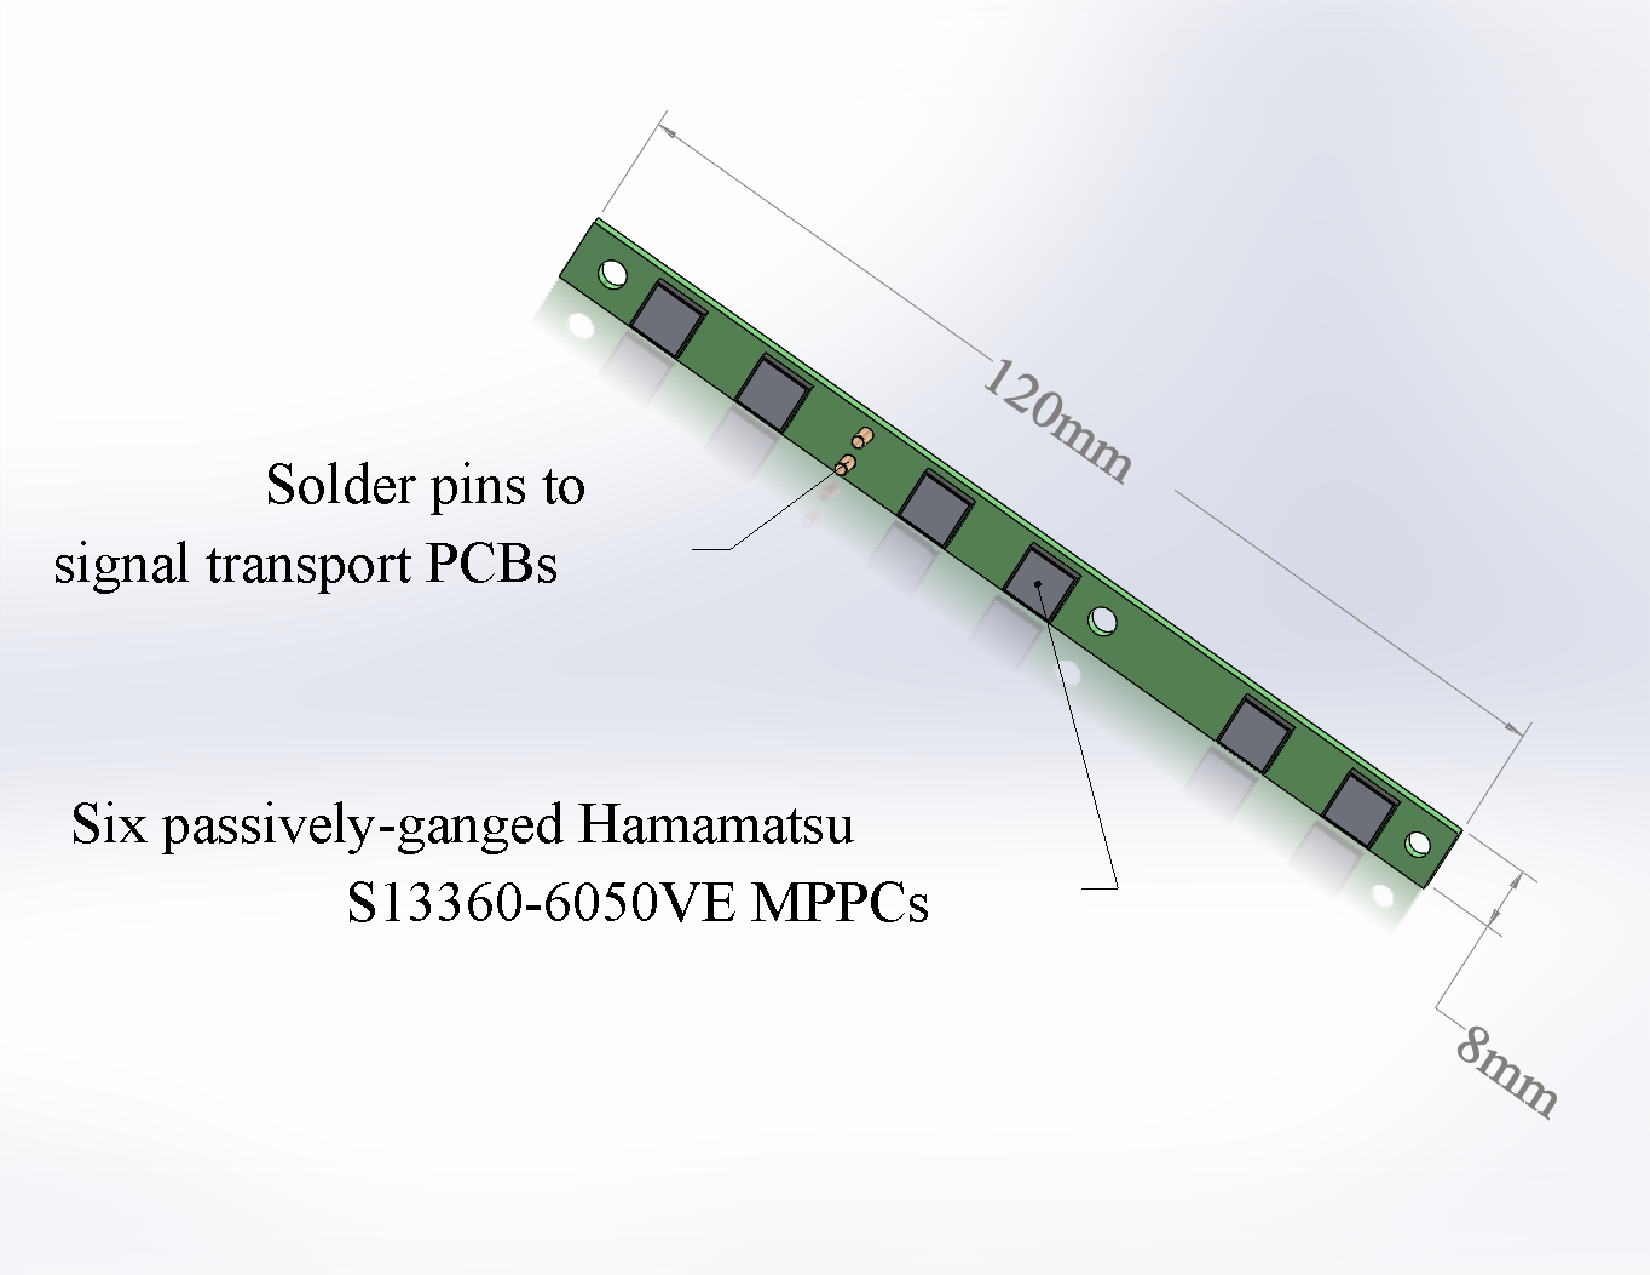
\includegraphics[height=7cm]{graphics/pds-photosensor-mounting-board-r4}
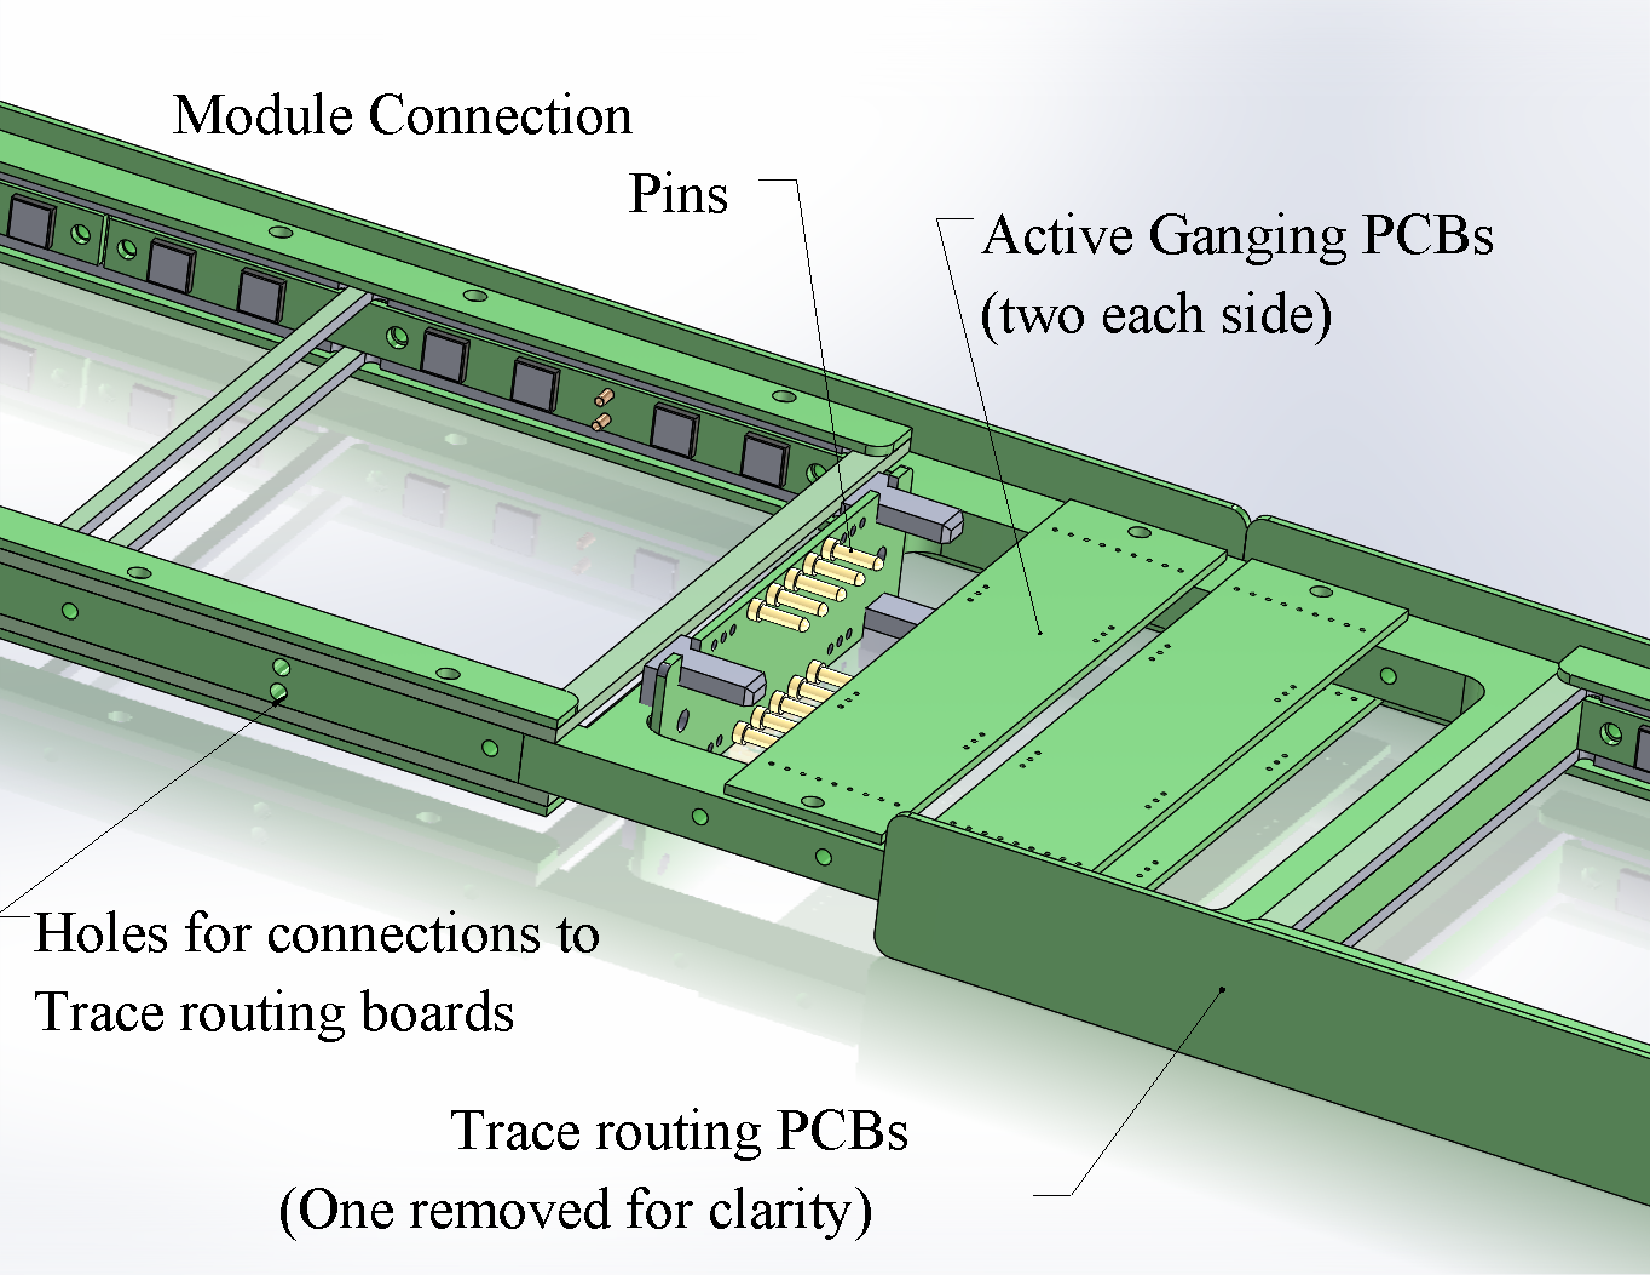
\includegraphics[height=7cm]{graphics/pds-trace-routing-pcb-r2}
\end{dunefigure}
The passively ganged signals are then routed through these boards to an active-ganging \dword{pcb} at the center of the module, where all eight passively ganged signals from a single supercell are actively ganged into one output channel (Figure~\ref{fig:mounting-board-routing-board}~(bottom)). This summed output from a single supercell is then connected to a single twisted pair in the Cat-6 readout cable for the module.  The active ganging \dwords{pcb} (one per supercell, four per module) are positioned in the module so that they are located inside the central \dword{apa} mechanical support tube when fully installed.


The  internal surface on the lateral sides of the cell are lined with the Vikuiti\texttrademark\ adhesive-backed dielectric mirror foil
that has been laser cut with openings at the locations of the \dwords{sipm} (i.e., the \dword{pcb} surfaces surrounding the \dwords{sipm} visible in Figure~\ref{fig:mounting-board-routing-board} will be highly-reflective).  In the case of the single-sided readout, the dichroic filter windows on the non-active side of the cell are replaced by a blank \frfour G-10 sheet lined in the cell interior with a Vikuiti\texttrademark\ reflector foil.
These types of foils have been used extensively in the WArP\footnote{Wimp ARgon Program at Gran Sasso: \url{http://warp.lngs.infn.it/}} and \dword{lariat}\footnote{Liquid Argon Time Projection Chamber at \dword{fnal}: \url{https://lariat.fnal.gov/}} experiments, where they performed well optically; no issues were reported related to adhesion of the film or dissolution of the wavelength shifter in \dword{lar}.

In \dword{dune}, we have demonstrated that the foils adhere very strongly to \frfour G10 surfaces cleaned following the \dword{pd} standard cleaning procedures.  Tests by the \dword{pd} group have demonstrated adhesion is maintained through multiple cryogenic (\dword{ln})/warm thermal cycles.  The mechanical design provides additional mechanical constraints on the Vikuiti\texttrademark\ sheets after module assembly, so the foils will be held in place mechanically even if the adhesive fails.  Samples of the adhesive have been used in other experiments with no negative impact on the \dword{lar} purity observed.  Samples will be tested in the \dword{fnal} materials test stand, and in \dword{iceberg}, \dword{sbnd}, and \dword{pdsp2} to confirm that the adhesive does not negatively impact \dword{lar} purity or detector performance.

To allow for air to vent out of the cell and \dword{lar} to completely fill the cell during the detector fill, holes are provided at the end of each supercell (four holes total, top and bottom of the cell when mounted in the \dword{apa}s).

The optical window(s) of each supercell are dichroic filters with a cut-off at \SI{400}{nm}. While the filters used for the \dword{pdsp} prototypes have been acquired from Omega Optical Inc.\footnote{Omega Optical Inc., Brattleboro, VT USA: \url{http://www.omegafilters.com/}}, Opto Eletronica S.A.\footnote{Opto Electronica S.A.: \url{http://www.opto.com.br/}} (in Brazil) is our current primary candidate vendor for \dword{dune} production filters.  Opto is a well-established company with a long history of involvement in research optical components for harsh environments and large thermal gradients (including camera optics for satellite photography).  We plan an extensive suite of testing of their filters at \dword{unicamp}, in \dword{iceberg}, and in \dword{pdsp2}. Other vendors are also being investigated\footnote{ASHAI -Japan, Andover-USA, and Edmunds Optics-USA}.

The filters are coated on the external side facing the \dword{lar} active volume with \dword{ptp}\footnote{p-TerPhenyl, supplier: Sigma-Aldrich\textregistered.}.  The coatings for the \dword{pdsp} modules have been made at the thin film facility facility at \dword{fnal} using a vacuum evaporator. Each coated filter was dipped in \dword{ln} to check the stability of the evaporated coating at cryogenic temperature. 

For the \dword{fd}, filter coatings will be done by the vacuum deposition facility at \dword{unicamp} (see Section~\ref{sec:xarapuca-unicamp}).

\section{Silicon Photosensors} %%%%%%%%%%% 1/8/20 Anne%%%
\label{sec:fdsp-pd-ps}

The physics goals, the design of the light collectors, and the trigger and \dword{daq} system constraints determine the suite of specifications for the silicon photosensors such as the number of devices, spectral sensitivity, dynamic range, triggering threshold and rate, and zero-suppression threshold. An initial survey of commercial products and a 12-month period of R\&D indicated that the performance characteristics of devices from several vendors effectively meet the \dword{pds} needs. 
However, a key additional requirement is to ensure the mechanical and electrical integrity of these devices in a cryogenic environment. Catalog devices for most vendors are certified for operation only down to \num{-40}$^\circ$C and though one candidate device performed well initially, after an unadvertised production process change a large fraction cracked when submerged in \dword{lar}\footnote{SensL MicroFC-60035C-SMT}. This highlighted the need to be in close communication with vendors in the 
\dword{sipm} design, fabrication, and packaging certification stages to ensure 
robust and reliable long-term operation in a cryogenic environment. 

Nearly one thousand \dwords{sipm}, of several types, are used in \dword{pdsp}'s \dword{pds}\footnote{\dword{pdsp} uses 516 SensL MicroFC-60035C-SMT, 288 Hamamatsu MPPC 13360-6050CQ-SMD with cryogenic packaging, and 180 Hamamatsu MPPC 13360-6050VE.}, providing an excellent test bed for evaluation and monitoring of \dword{sipm} performance in a realistic environment over a period of months. Results from \dword{pdsp} are summarized in Section~\ref{sec:fdsp-pd-validation}.

The \dword{spmod} baseline \dword{pds} design has \num{192} \num{6}$\times$\SI{6}{mm$^2$} \dwords{mppc} per \dword{pd} module with groups of \num{48} \dwords{mppc} electrically ganged into four electronics readout channels. This leads to a total of \num{288000} \dwords{mppc}. % per \dword{spmod}. 

Two entities have expressed interest to engage with the consortium with an explicit intent to provide a product specifically for cryogenic operation: (1) Hamamatsu Photonics K.K., a large well-known commercial vendor in Japan, and (2) \dword{fbk}\footnote{Hamamatsu Photonics K.K.: \url{https://www.fbk.eu/en/}}
in Italy. 
\dword{fbk} is an experienced developer of solid state photosensors that typically licenses its technology; it is partnering with the DarkSide\footnote{Darkside project: \url{http://darkside.lngs.infn.it/}} collaboration to develop devices with specifications very similar to \dword{dune}'s.  Table~\ref{tab:photosensors} summarizes the key characteristics of the baseline device, Hamamatsu S13360, and two other devices from Hamamatsu and \dword{fbk} that are under consideration.

While the devices from Hamamatsu have been tested extensively by the consortium, those from \dword{fbk} are relatively new to us. The technologies they have developed that are suitable for the needs of \dword{dune} are the NUV-HD-SF (standard field) and NUV-HD-LF (low field)~\cite{Gola:2019idb}. In particular, the LF technology (see Table~\ref{tab:photosensors}) offers the lowest dark current rate and has been successfully employed for the DarkSide experiment. NUV-HV-SF sensors developed by \dword{fbk} specifically for \dword{dune} have been tested in Milano (Italy), CSU (CO, US), and NIU (IL, US). The sensors were characterized both at room and cryogenic temperatures (\SI{77}{K}) and underwent more than \num{50} thermal cycles. The tests confirmed the nominal performance of the photosensors and proved the reliability of the sensors at low temperature. Extensive thermal tests and characterization of sensors in the NUV-HD-LF technology are in progress.   

The milestone for photosensor selection for the first \dword{spmod} is early 2021.  Though a baseline photosensor that meets the requirements has been identified, the addition of experienced INFN groups to the \dword{pds} effort has enabled us to pursue the promising \dword{fbk} option in a way that was not possible previously.  We are carrying out targeted investigations on the performance, cost, and production capability to establish the viability of the alternatives for all or part of the sensors required for either the first or subsequent \dwords{spmod}. Two photosensor types (one from each vendor) will be selected in early 2020 to be used in \Dword{pdsp2}.

As described in Section~\ref{sec:fdsp-pd-lc}, the size and sensitivity of currently available \dwords{sipm} requires that multiple devices are needed for each \dword{xarapu} cell. The spatial granularity of each device is much smaller than required for \dword{dune} so,
along with limitations on the number of readout channels, it is required that the signal output of the \dwords{sipm} must be electrically ganged. The terminal capacitance of the sensors strongly affects the \dword{s/n} when devices are ganged in parallel, which led to a design that passively gangs several sets of \dwords{sipm} in parallel, which are then summed with active components, as described in Section~\ref{sec:pds-design-ganging}.


\begin{dunetable}[Candidate photosensors characteristics]
%{p{0.18\textwidth}p{0.18\textwidth}p{0.18\textwidth}p{0.18\textwidth}}
{p{0.26\textwidth}p{0.26\textwidth}p{0.18\textwidth}p{0.18\textwidth}}
{tab:photosensors}
{Candidate Photosensors Characteristics.}
	                      &Hamamatsu (Baseline)   & Hamamatsu-2    & FBK                 \\ \toprowrule
Series part \#            & S13360                &     S14160         & NUV-HD-LF         \\ \colhline
V$_{\rm br}$ (typical)    & 50 V to 52 V          &   36 V to 38 V & 31 V to 33 V                \\ \colhline
V$_{\rm op}$ (typical)    & V$_{\rm br}$+\SI{3}{V}             &   V$_{\rm br}$+\SI{2.5}{V} & V$_{\rm br}$+\SI{3}{V}                \\ \colhline
Temperature dependence of V$_{\rm br}$  & \SI{54}{mV/K}&  \SI{35}{mV/K}& \SI{25}{mV/K}   \\ \colhline
Gain~at~V$_{\rm op}$(typical)   & $1.7\times10^6$     &      $2.5\times10^6$ &  $0.75\times10^6$          \\ \colhline
Pixel size                & 50 $\mu$m             &       50 $\mu$m    & 25 $\mu$m            \\ \colhline
Size                      & 6 mm x 6 mm           &     6 mm x 6 mm    & 4 mm x 4 mm            \\ \colhline
Wavelength                & 320 to 900 nm         &     280 to 900 nm  & 280 to 700 nm            \\ \colhline
PDE peak wavelength       & \SI{450}{nm}         &      \SI{450}{nm}     & \SI{450}{nm}           \\ \colhline
PDE at peak                & 40\%                  &        50\%        & 50\%            \\ \colhline
DCR at \si{0.5}{PE}               & < \SI{50}{\kilo\hertz\per\square\milli\meter}      & < \SI{100}{\kilo\hertz\per\square\milli\meter}   & < \SI{25}{\kilo\hertz\per\square\milli\meter}               \\ \colhline
Crosstalk                 & <~3\%				  &      <~7\%          & <~3\%             \\ \colhline
%Afterpulsing              &                       &                &                 \\ \colhline
Terminal capacitance      & \SI{35}{\pico\farad\per\square\milli\meter}          &   \SI{55}{\pico\farad\per\square\milli\meter}     &      \SI{50}{\pico\farad\per\square\milli\meter}         \\ \colhline
Lab experience            & Mu2e and DUNE prototypes      &                &     Darkside  \\         
\end{dunetable}


%%%%ELECTRONICS %%%%%%%%%%%%%%%%%%%%%%%%%%%%%%%%%%%%%%%%%%%%%%%%%%%

\section{Electronics}
\label{sec:fdsp-pd-pde}
%\metainfo{\color{red}\bf  Content: Djurcic/Franchi/Moreno/Spitz/Toups}

The electronic readout system for the \dword{pds} must (1) collect and process electrical signals from \dword{sipm}s reading out the light collected by the \dwords{xarapu}, (2) provide an interface with the trigger and timing systems supporting data reduction and classification, and (3) transfer data to offline storage for physics analysis. Figure~\ref{fig:pds-electronics_signalpath} provides a simple overview of the signal path and key elements. 
\begin{dunefigure}[Overview of the \dshort{pds} signal path]
 {fig:pds-electronics_signalpath}
 {Overview of the \dword{pds} signal path.}
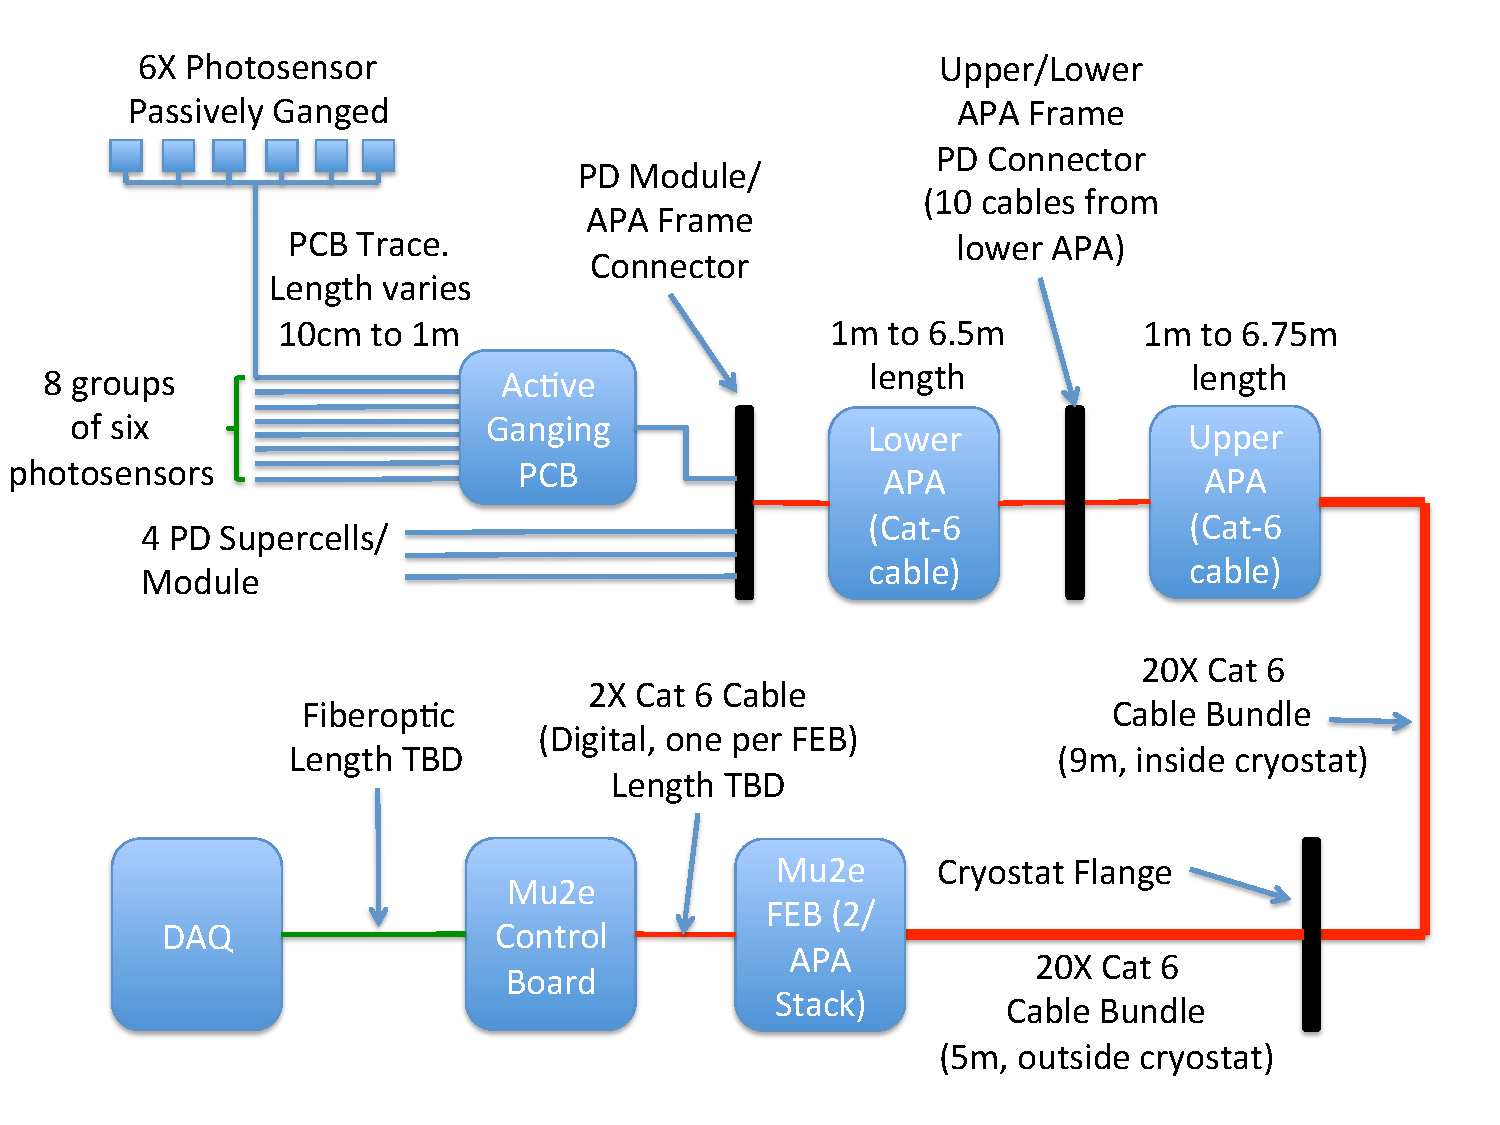
\includegraphics[width=15cm]{graphics/pds-signal-routing-diagram-r3.pdf}
\end{dunefigure}


As specified in the requirements Table~\ref{tab:specs:SP-PDS}, the readout system must enable the $t_0$ measurement of non-beam events; this capability will also enhance beam physics by recording interaction time of events within 
beam spill more precisely to help separate against potential cosmic background interactions. A highly capable readout system was developed for use with \dword{pdsp} and prototype development as described in Section~\ref{sec:valid-pdsp}. However, a more cost-effective waveform digitization system developed for the \dword{mu2e} experiment has been identified and selected as the baseline choice for the \dword{pd} system. 


\subsection{SiPM Signal Ganging}
\label{sec:pds-design-ganging}

The ganging of electrical signals from \dword{sipm} arrays is implemented to minimize the electronics channel count while maintaining adequate redundancy and granularity, as well as to improve the readout system performance.  
Technical factors that affect performance of the ganging system are the characteristic capacitance of the \dword{sipm} and the number of \dwords{sipm} connected together, which together dictate the \dword{s/n} and affect the system performance and design considerations.

We have demonstrated a feasible purely passive summing scheme with twelve Hamamatsu \dword{mppc} sensors now operational in \dword{pdsp}. For optimal performance in \dword{dune}, we have shown that an ensemble of 48 Hamamatsu \SI{6}{mm}$\times$\SI{6}{mm} \dwords{mppc} can be summed into a single channel by a combination of passive and active ganging (see Section~\ref{sec:pds-valid-ganging}).  In this scheme, an amplifier is used to adjust the \dword{mppc} output signal level to the input of an \dword{adc}; the active summing is realized with an OpAmp THS4131. This combination of passive and active ganging with cold signal summing and amplification, illustrated in Figure~\ref{fig:fig-pds-6x8gang}, is the baseline for the \dword{pds}.

\begin{dunefigure}[SiPM signal summing board circuit]
 {fig:fig-pds-6x8gang}
 {\dword{sipm} signal summing board circuit: 6 passive  x 8 active, 48 \dwords{sipm} total.}
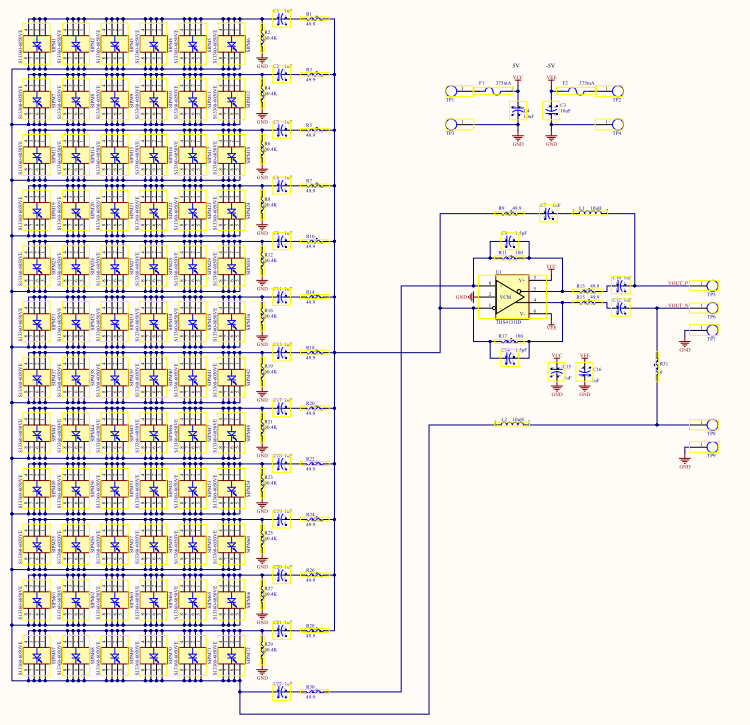
\includegraphics[height=14cm]{graphics/pds_gang_fig2.png}
\end{dunefigure}

%%%%%%%%%%%%%%%%%%%%%%%%%%%%%%%%%%%%%%%%%%%%%%%%%%%%%%%%%%%%%%%%

\subsection{Front-end Electronics Baseline Design}
\label{sec:electronics}

The \dword{fe} electronics for the development and prototype stages of the  \dword{pds}, including \dword{pdsp}, was provided by a custom-designed \dword{sipm} Signal Processor (\dword{ssp}, see \citedocdb{3126}). This system was highly configurable and provided detailed information on the photosensor signal, which allowed a thorough understanding of the photon system performance.
For the much larger \dword{spmod}, a system is required that meets the performance requirements yet optimizes the cost.
To this end, we have developed a solution based on lower-sampling-rate commercial ultrasound \dword{asic} chips rather than digitizers based on flash \dwords{adc} used in the \dword{ssp}. Inspiration for this cost-effective \dword{fe} comes from the system developed for the \dword{mu2e} experiment cosmic ray tagger readout system.
Both \dword{ssp} and the new design are used in the \dword{pd} validation process summarized in Section~\ref{sec:fdsp-pd-validation} to allow direct comparison.

Development of the readout electronics to date has been primarily by US groups. 
However, since fabrication of the \dword{dune} readout electronics will be conducted by a collaboration of Latin American institutions (including groups in Peru, Colombia, Paraguay, and Brazil), further development is being performed by these groups, with support from the US groups.  
The engineers met and worked together at \dword{fnal} in summer 2019, and that collaboration is continuing.  We expect the first \dword{daphne} prototypes to be complete and tested in \dword{iceberg} in April/May 2020.  
%Engineers from several of the groups will meet at \dword{fnal} in the summer of 2019 to continue the development of the system. The \dword{iceberg} facility at \dword{fnal} will provide a realistic system test of the prototypes.  
Pre-production \dword{mu2e}-based electronics readout will also be tested in the \dword{pdsp2} run at \dword{cern} in 2021-2022.


\subsubsection{Front-end Board and Controller}

The readout and digitization of the signals from the active summing board described in Section~\ref{sec:pds-design-ganging} will rely on a set of \dword{fe} board (\dword{feb}) readout electronics boards and controller boards, originally designed for the \dword{mu2e} experiment~\cite{bib:mu2e_tdr}
at \dword{fnal}. As discussed in Section~\ref{sec:pds-valid-ganging}, preliminary results indicate that the active-summing board and \dword{mu2e} electronics \dword{feb} combination will perform well together and, in general, meet the readout requirements for the experiment. Figure~\ref{fig:feb} shows the 64~channel \dword{feb} design carried over from \dword{mu2e}. The board has a number of notable features, discussed below. Most importantly,  
the board is designed to utilize commercial, off-the-shelf parts only, and is therefore quite inexpensive compared to other designs. In particular, the digitization implements the low-noise, high-gain, and high-dynamic-range commercial \dwords{adc} used in ultrasonic transducers. 

The \dword{feb} is the centerpiece of the baseline readout electronics system.  
The current 64~channel\footnote{This text assumes 64 channels/\dword{feb} when presenting the \dword{feb} and controller. However, we envision 40~channels/\dword{feb} in the final design, corresponding to a single \dword{apa} as described in Section~\ref{subsec:pds-fe-next}.} \dword{feb} relies on commercial ultrasound chips\footnote{Texas Instruments\texttrademark{} 12~bit, 80~megasamples/s (MS/s); AFE5807.},
with programmable anti-alias filters and gain stages, to read out the \dword{mppc} signals from the active ganging boards inside the \dword{pd} modules. The board currently takes HDMI inputs, with four channels per input.  Each of the eight ultrasound chips on an \dword{feb} handles eight channels (\SI{120}{mW} per channel) of data using a low-noise preamplifier, a programmable gain amplifier, and a programmable low-pass filter. The information is buffered with a total of \SI{1}{GB} DDR SDRAM, divided in four places, and a set of Spartan~6\texttrademark~\dwords{fpga} are used for parallelizing the serial \dword{adc} data, zero suppression, and timing. Each of the four \dwords{fpga} on a board, corresponding to 16 channels, handles two \dword{adc} chips with an available \SI{256}{MB} DDR SDRAM. 

After digitization, the data from each \dword{feb}, in the form of pulses (time-stamp and pulse height), is sent via Ethernet to a master controller that aggregates the signals from 24 \dword{feb}s, or $64\times24=1536$ channels. The 24 \dword{feb}s corresponding to a single controller will come in sets of 12, with each set of 12 \dword{feb}s referenced to a single chassis as shown in %. A picture and schematic of the controller is seen in 
Figure~\ref{fig:controller}. A trigger decision (e.g., accelerator timing signal) can be produced and/or received by the controller and, depending on the decision, each event's digital information is sent to the controller and then to \dword{daq} computers for processing and storage. The controller-to-\dword{daq} connection will rely on a fiber connection, although an Ethernet-based controller output option is available.

\subsubsection{Bandwidth, readout rates, and zero suppression}

\dword{daq} system and data storage limitations impose constraints on the  data flow from the \dword{fe} electronics system. 
For example, if it were necessary to read out a \SI{5.5}{\micro\second} waveform in order to include more of the longer time constant scintillation light component, the \SI{80}{megasamples/s} (MS/s), 12-bit \dword{adc} device would produce a \SI{5.3}{kbit} waveform. For an envisioned dark count (DC) rate of 250~Hz/channel, this corresponds to a data transfer rate of \SI{53}{MB/s}/\dword{apa} (1~\dword{apa}=40 channels) or \SI{6.6}{MB/s} \dword{feb}-to-controller DC rate. This rate approaches the crucial bottleneck in the electronics readout system with a maximum rate of \SI{10}{MB/s} (per \dword{feb}). However, zero-suppression techniques and multi-channel coincidence/threshold requirements at the \dword{feb} firmware level can be used to significantly mitigate this issue, noting that each on-\dword{feb} \dword{fpga} handles 16 channels. 

The design is flexible enough to accommodate modest changes in system requirements, such as the suppression factor determined by parameters like the readout window length and limits on the overall trigger rate. 
Firmware and zero-suppression technique development is in progress and can easily adapt to the physics and calibration requirements of the \dword{pd}.
In addition to its bandwidth and DC rate readout capabilities, the system can also  manage a highly coincident event in which a large number (or all) channels fire at once. 
For example, the controllers' 24-board write speed of \SI{150}{MB/s} could handle even the unlikely all-detector event featuring 6000~channels firing at once (corresponding to \SI{4}{MB} event size). 

The baseline electronics readout system performance is consistent with the \dword{daq} interface specification of \SI{8}{Gb/s} per connection, given that
each \dword{feb} signal corresponds to a maximum of \SI{10}{MB/s} (\SI{240}{MB/s} total).  

\subsubsection{Power, grounding, and rack schemes} 

Figure~\ref{fig:grounding_power} shows the grounding, power, and data link schemes for the system. The \dword{feb}s are powered via power-over-Ethernet (\SI{600}{mA}, \SI{48}{V} supply) from the controller. One Cat-6 cable from the controller to each \dword{feb} handles the signal and power simultaneously. The reference planes of the controller and \dword{feb} are isolated on both sides. The grounding scheme calls for each set of twelve \dword{feb}s referenced to a single chassis, with each chassis and corresponding controller on detector ground and the \dword{daq}, connected to each controller via fiber, on building ground. 
 
The rack space and power consumption required by the system assume
a total of 6000 channels with 40 channels/\dword{feb}. This system requires 13 chassis (12 \dword{feb}/chassis) at 6U each and seven controllers (controlling 24 \dword{feb} each) at 1U each; these can be accommodated in just over two 42U capacity racks. The power supply on a controller is \SI{700}{W}, with each \dword{feb} taking \SI{20}{W}. 
 

\begin{dunefigure}[\dshort{pds} 64-channel front-end board]
 {fig:feb}
 {Photograph of the 64-channel \dword{pds} \dword{fe} board (\SI{80}{MS/s}, \SI{12}{bit} ADC) (left); schematic of the \dword{fe} board (right).}
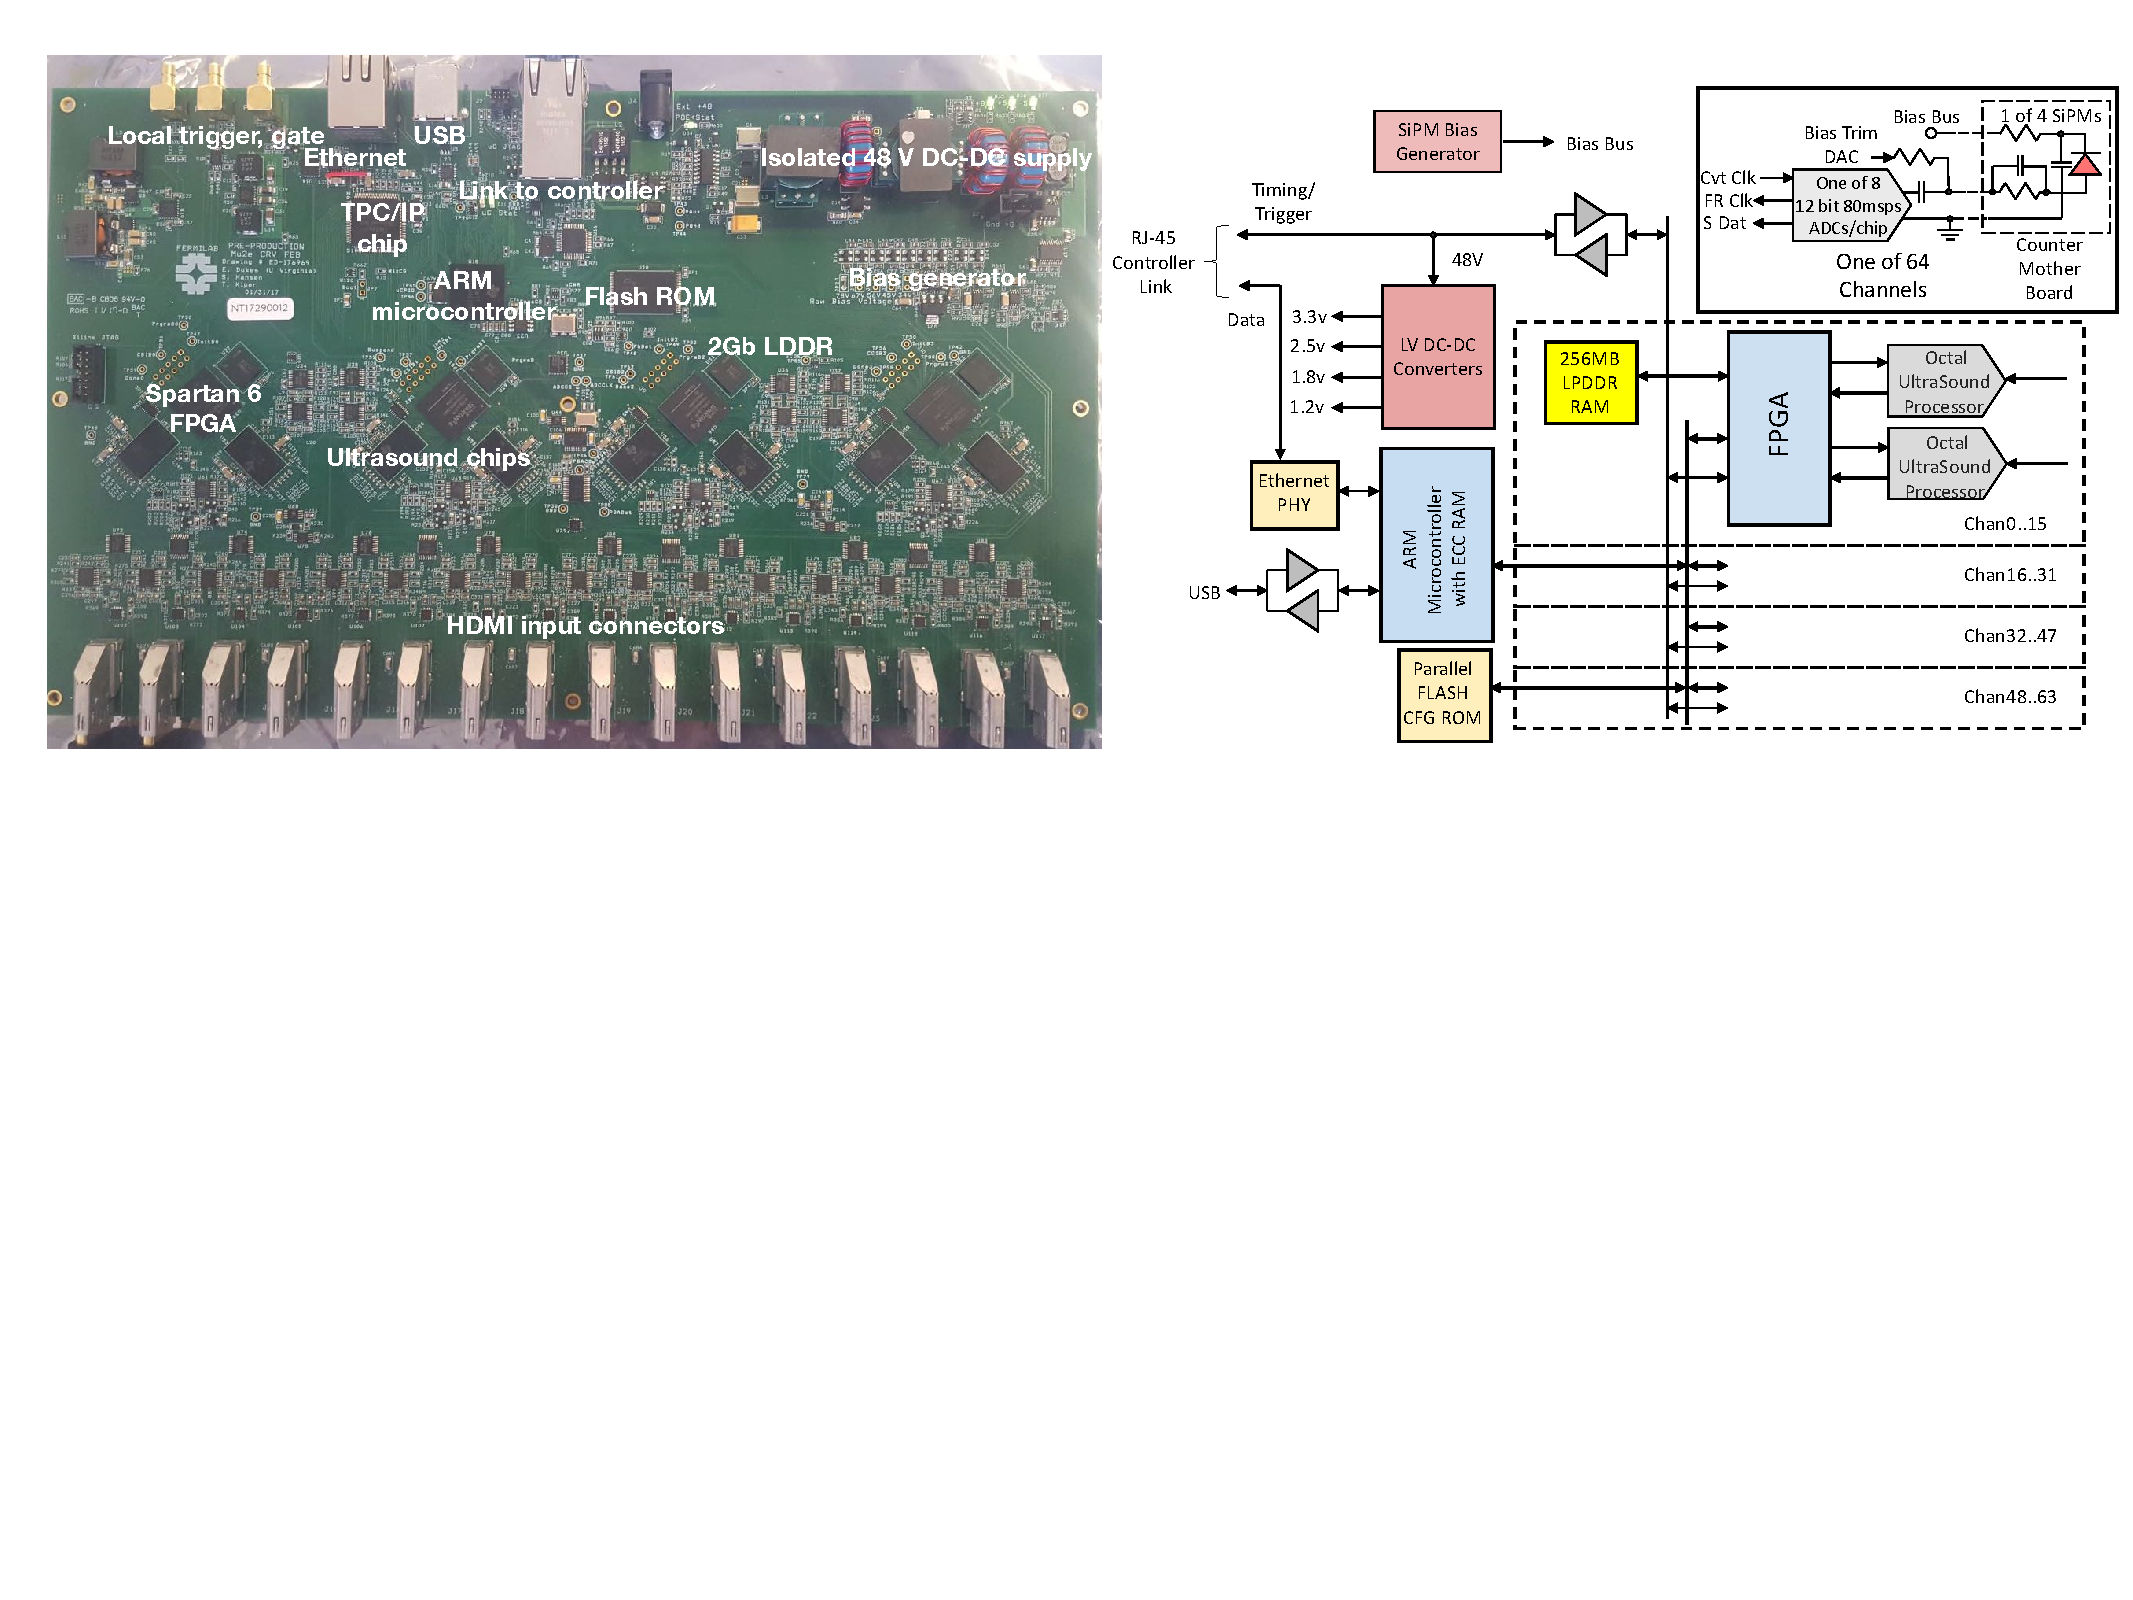
\includegraphics[height=5.2in]{graphics/pds-feb-tdr.pdf} 
\vspace{-6.3cm}
\end{dunefigure}

\begin{dunefigure}[\dshort{pds} front-end electronics controller module]
 {fig:controller}
 {The front (left-bottom) and back views of the controller module (left-top); it is capable of accepting signals from 24 \dword{feb}s; schematic of the controller (right).}
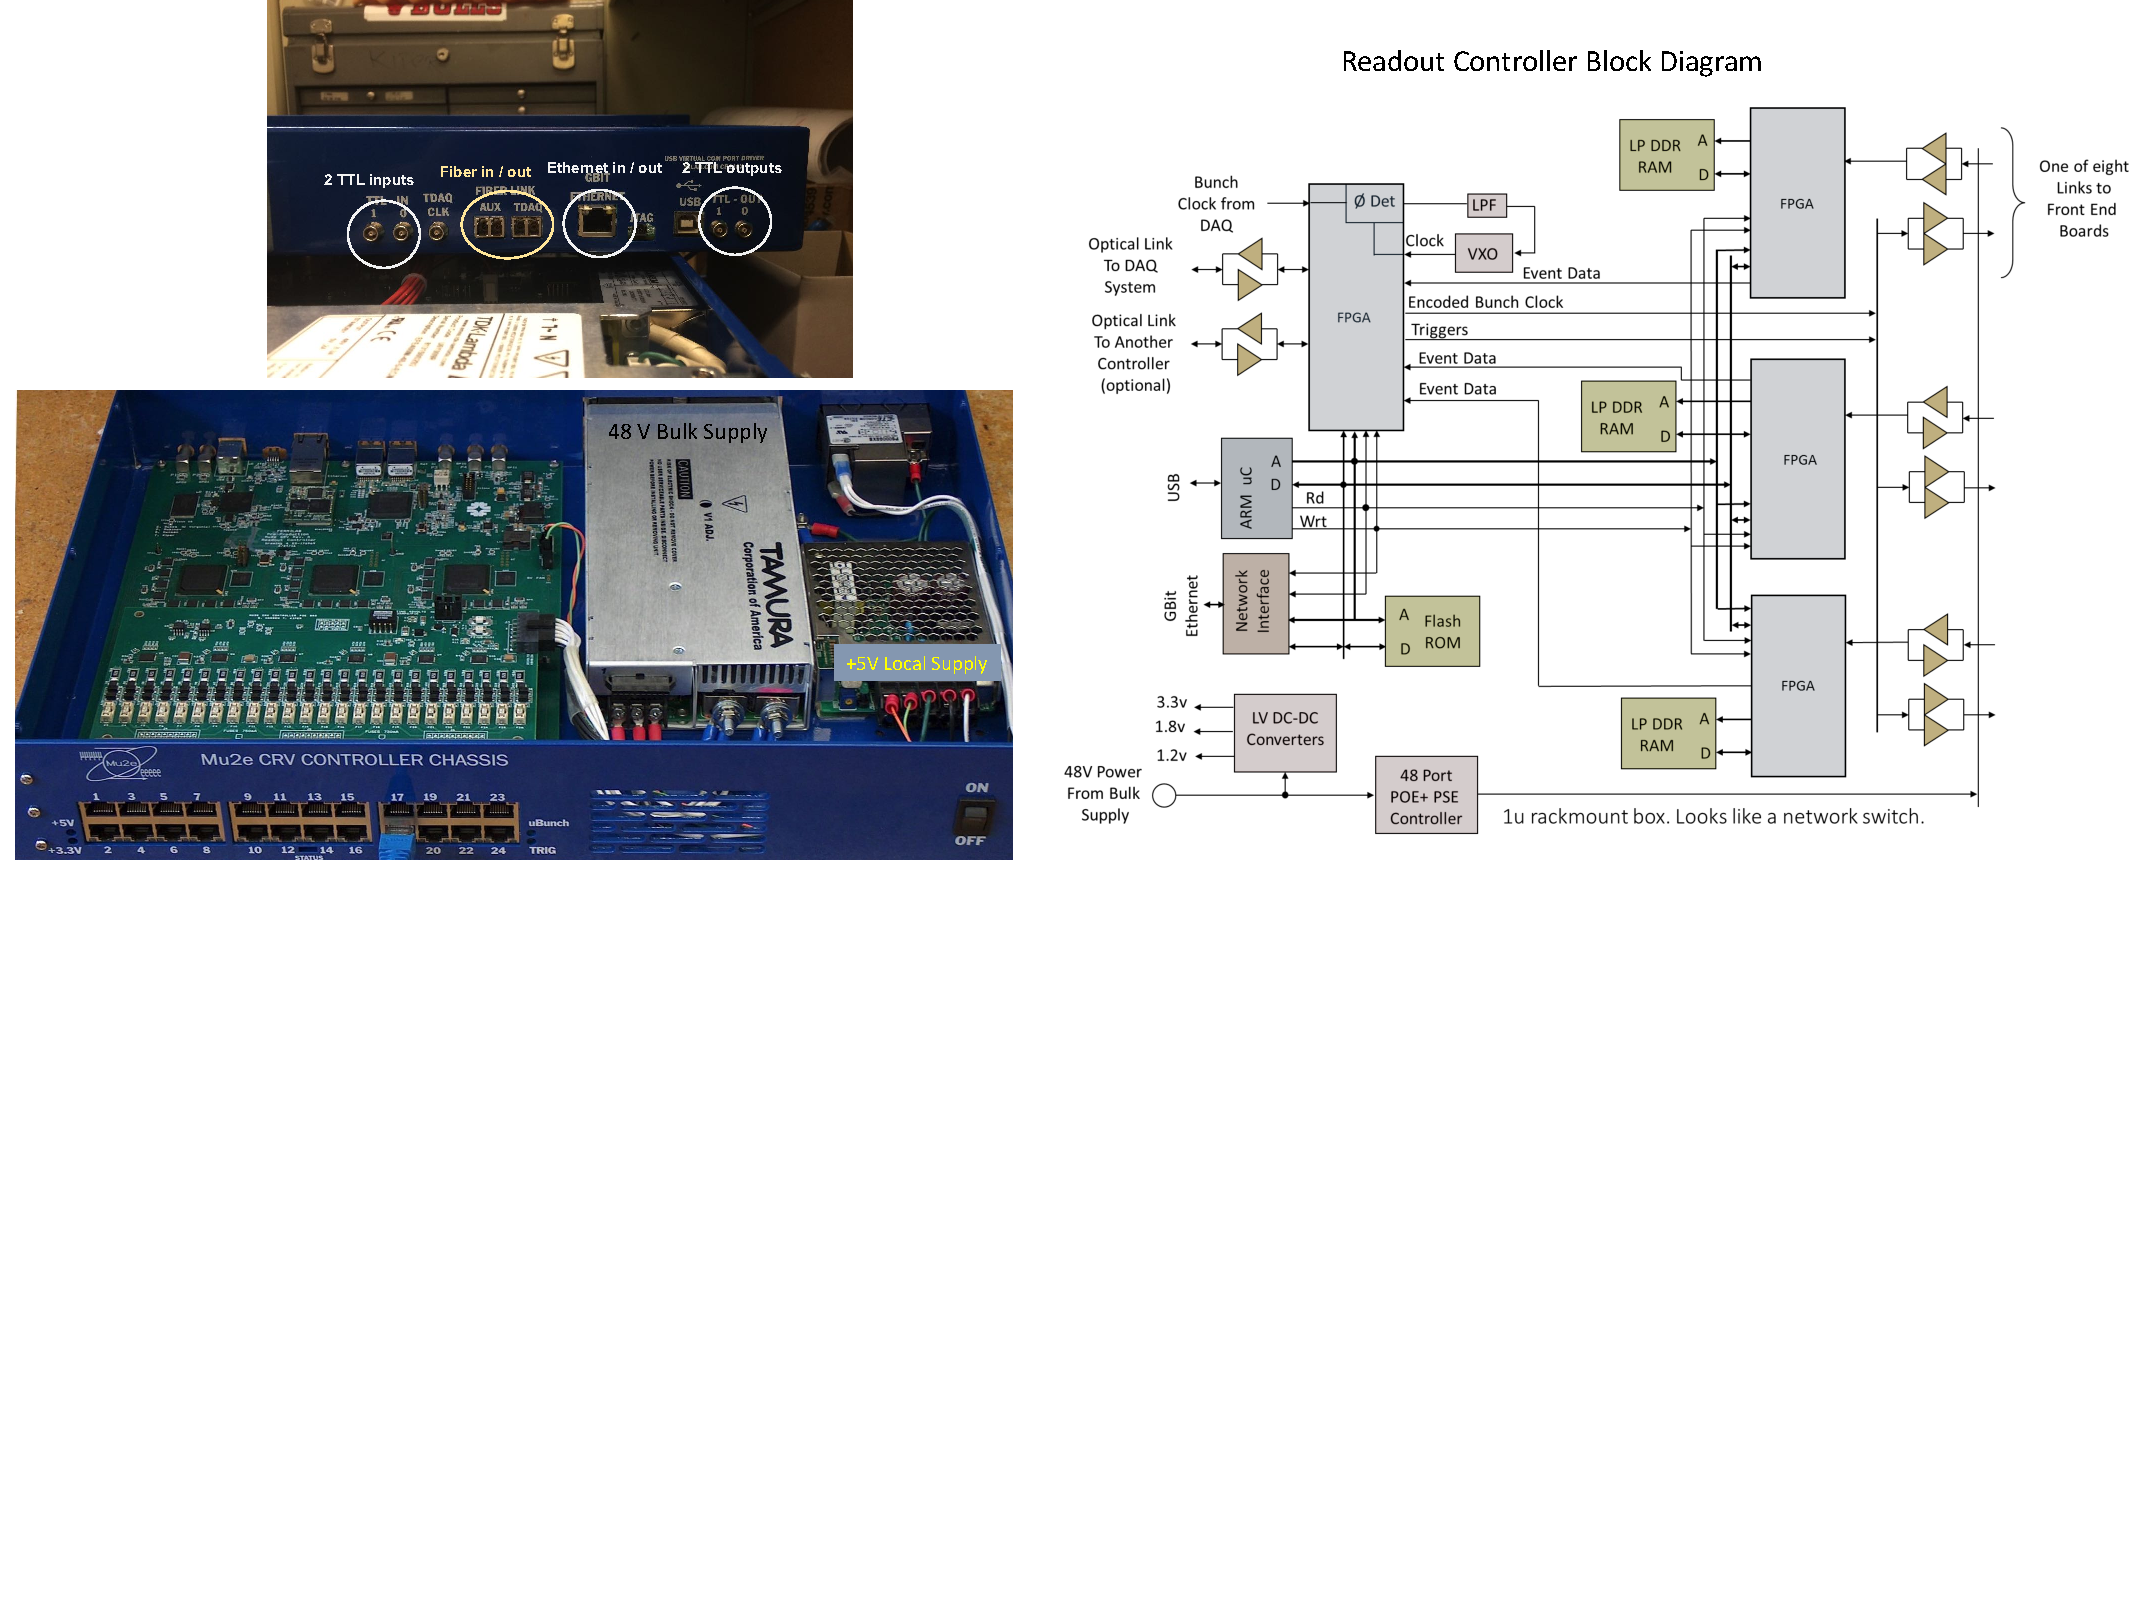
\includegraphics[height=5.1in]{graphics/pds-controller.pdf} 
\vspace{-5.5cm}
\end{dunefigure}

\begin{dunefigure}[\dshort{pds} front-end electronics grounding scheme]
 {fig:grounding_power}
 {Grounding scheme with 1 chassis, containing 12 \dword{feb}s, a controller module, and a \dword{daq} PC, as an example (left); power and data link arrangement of the \dword{feb} and controller (right).}
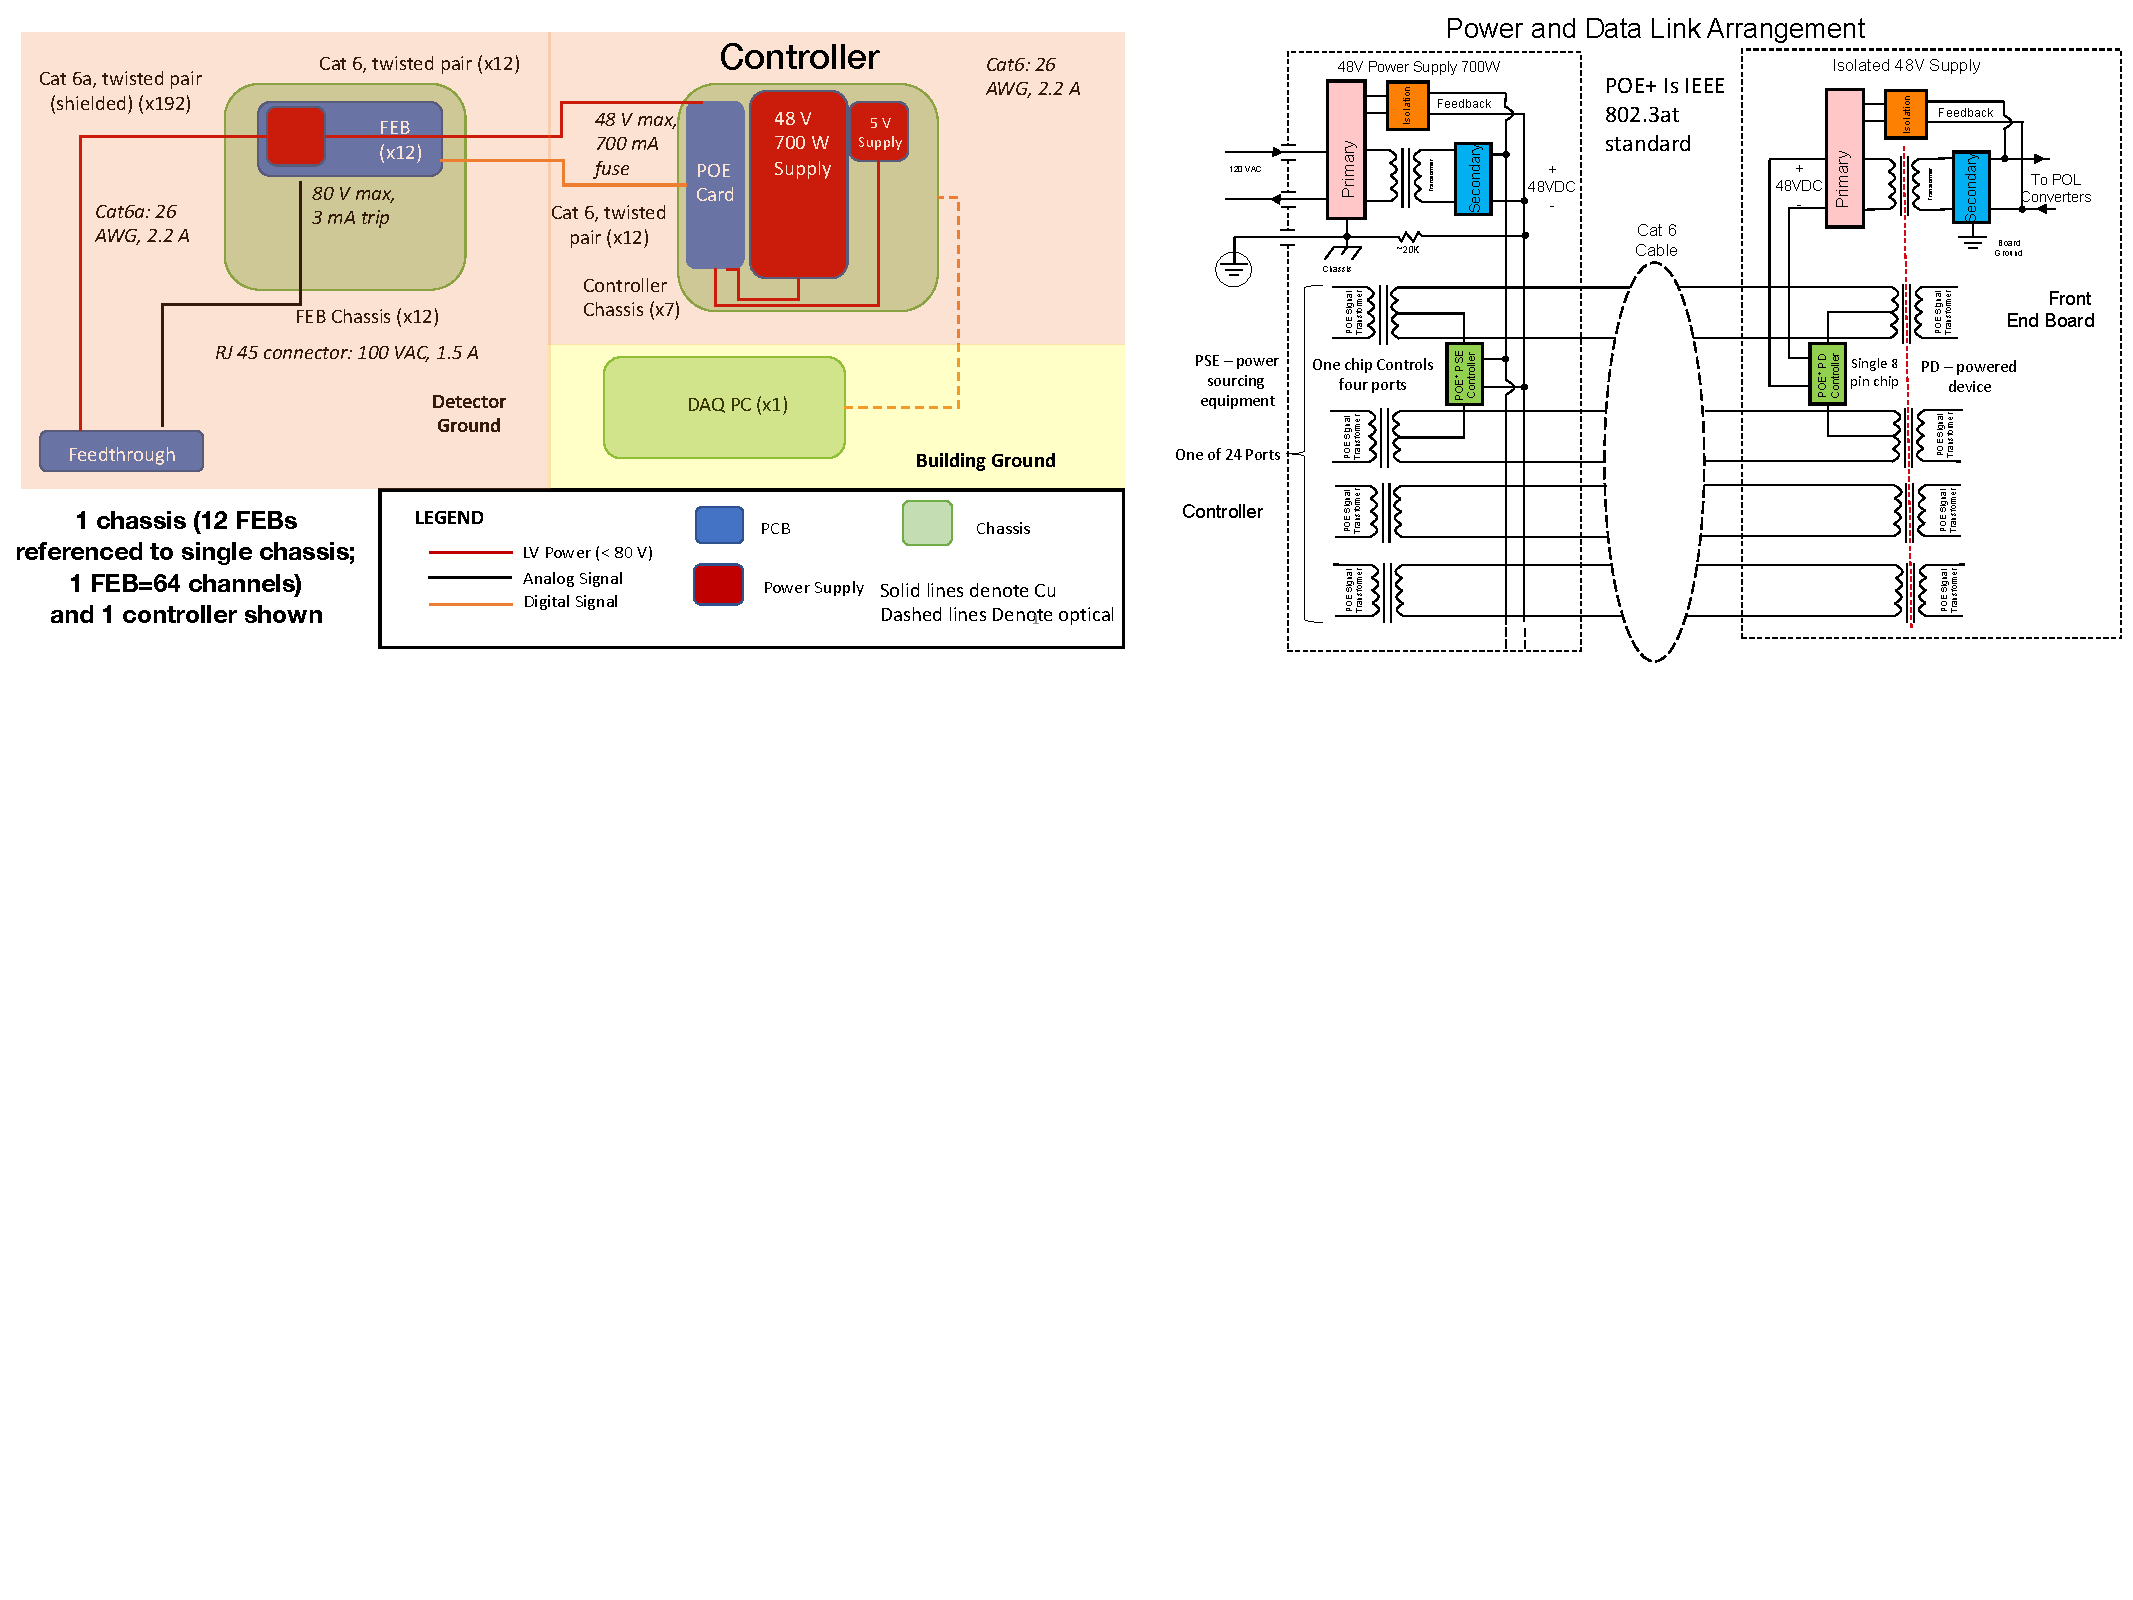
\includegraphics[height=5.0in]{graphics/pds-grounding-power.pdf} 
\vspace{-7.1cm}
\end{dunefigure}

\subsection{Electronics Next Steps}
\label{subsec:pds-fe-next}


The \dword{feb}s, developed for the \dword{mu2e} cosmic ray veto and proposed for use in \dword{dune}, can read out an array of \dwords{mppc} with an adequate \dword{s/n} ration to be sensitive to single photons. However, we want to optimize and further develop them by pursuing the following tasks:

\begin{enumerate}
\item To better match the 40 \dword{pdsp} channels per \dword{apa}, the system presented here assumes that only 40 out of the 64 channels on the existing  \dword{mu2e} \dword{feb} are populated with active electronics.  A prototype board will test this configuration and validate the associated cost model.

\item The  \dword{mu2e} warm readout electronics use last-generation (Xilinx\texttrademark{} Spartan-6) \dwords{fpga} and other components that have since been superseded by newer devices.  Design and prototyping work will 
incorporate newer \dwords{fpga} (Xilinx Spartan-7 or Artix-7) into the electronics,
improving their performance and maintainability over the lifetime of the \dword{dune} experiment. The Artix-7 \dwords{fpga} have been implemented in the \dword{ssp} readout system used in \dword{pdsp}, and therefore the expertise with these system components has been established. 

\item Results from the  \dword{iceberg} test stand can determine whether there are sufficient logic resources in the \dwords{fpga} to meet a broad range of possible \dword{daq} requirements expected from the warm readout electronics. To that end, the low-cost \dword{fe} solution will be compared to existing \SI{14}{bit}, \SI{150}{MS/s} \dword{ssp} readout.  Straightforward zero suppression schemes that can be implemented on the Mu2e board with the current Spartan-6 \dword{fpga} will be tested with respect to potential \dword{daq} data rate limitations.  However, increases in the number of logic cells can be accommodated by switching to more capable, but still pinout-compatible, devices within the same Xilinx \dword{fpga} family as discussed above.

\item It may be desirable to increase the dynamic range of the \dwords{adc} used on the \dword{feb}s in order to achieve desired physics goals related to the energy resolution of beam neutrino events.  To this end, we plan to investigate replacing the TI AFE5807 ultrasound chip with the TI AFE5808 ultrasound chip, which is pinout-compatible but incorporates a 14-bit \dword{adc}.  Ultimately, a prototype board will incorporate all relevant optimizations and improvements.

\end{enumerate}

The final requirements for the system will be informed by analysis of the data from the readout system implemented in \dword{pdsp} and subsequent data from operating ICEBERG from August 2019 through the end of the year.

Additional testing of the system will continue through \dword{pdsp2} operations. The specifications for the readout electronics system will be reconsidered based on that experience and established before the \dword{pd} final design review (see the high-level schedule in Section~\ref{sec:fdsp-pd-org-cs}). 


%%%%%%%%%%%%%%%%%%%%%%%%%%%%%%%%%%%%%%%%%%%%%%%%%
\section{Calibration and Monitoring}
\label{sec:fdsp-pd-CandM}

Calibration and monitoring is an essential component of the \dword{pds}.
The primary system is a pulsed UV-light source that will allow calibration of the \dword{pd} gain, linearity, and timing resolution and monitoring the stability of the photon response of the system over time.
In many experiments, a pulsed light system is a valuable well-defined, controllable light source for monitoring but for (near) surface detectors, often a supplement to using tracked cosmic ray muons, which provide a much closer replica of the signal from events of interest. 
However, at \dword{dune}, the muon rate per individual photon detector will be very low and insufficient to monitor changes in the system response. In this situation, the pulsed system will play an essential role in achieving and maintaining the \dword{pd} performance required for neutrino calorimetry. 
This system will also be a valuable detector commissioning tool prior to sealing the cryostat, in the cool-down phase, and during the \dword{lar} fill.
Other complementary calibration systems, such as radioactive sources, are described in Chapter~\ref{ch:sp-calib}. 

The system design is almost identical to that deployed in \dword{pdsp}, as described in Section~\ref{sec:fdsp-pd-validation-candm}; the primary differences are the number of diffusers, the lengths of the optical fibers, and the addition of a monitoring diode.

The system hardware consists of both warm and cold components but has no active components within the cryostat. The active component consists of a 1U rack mount light calibration module (\dword{lcm}) located outside the cryostat. The \dword{lcm} generates UV (\SIrange{245}{280}{nm}) pulses that propagate through a quartz fiber-optic cable to diffusers at the \dword{cpa} that distribute the light uniformly across the \dwords{pd} mounted within the \dword{apa}. 
It consists of an \dword{fpga}-based control logic unit coupled to an internal \dword{led} pulser module (\dword{lpm}) and an additional bulk power supply. 
The \dword{lpm} has multiple digital outputs from the control board to control the pulse amplitude, pulse multiplicity, repetition rates, and pulse duration; programmable \dwords{dac} control the \dword{lpm} pulse amplitude. \dword{adc} channels internal to the \dword{lcm} are used to read out a reference photodiode used for pulse-by-pulse monitoring of the \dword{led} light output. The output of the monitoring diode is available for normalizing the response of the \dwords{sipm} in the detector to the monitoring pulse. 


\begin{dunefigure}[Calibration system diffuser locations on the SP CPA]
 {fig:pds-calmon-cpa-diffusers}
 {Schematic of a complete SP cathode plane ($\SI{60}{m}\times\SI{12}{m}$) showing the locations of the calibration and monitoring system diffusers. Each diffuser illuminates a region of about $\SI{4}{m}\times\SI{4}{m}$ (indicated by the squares) on \dword{apa}s \SI{3.6}{m} away.}
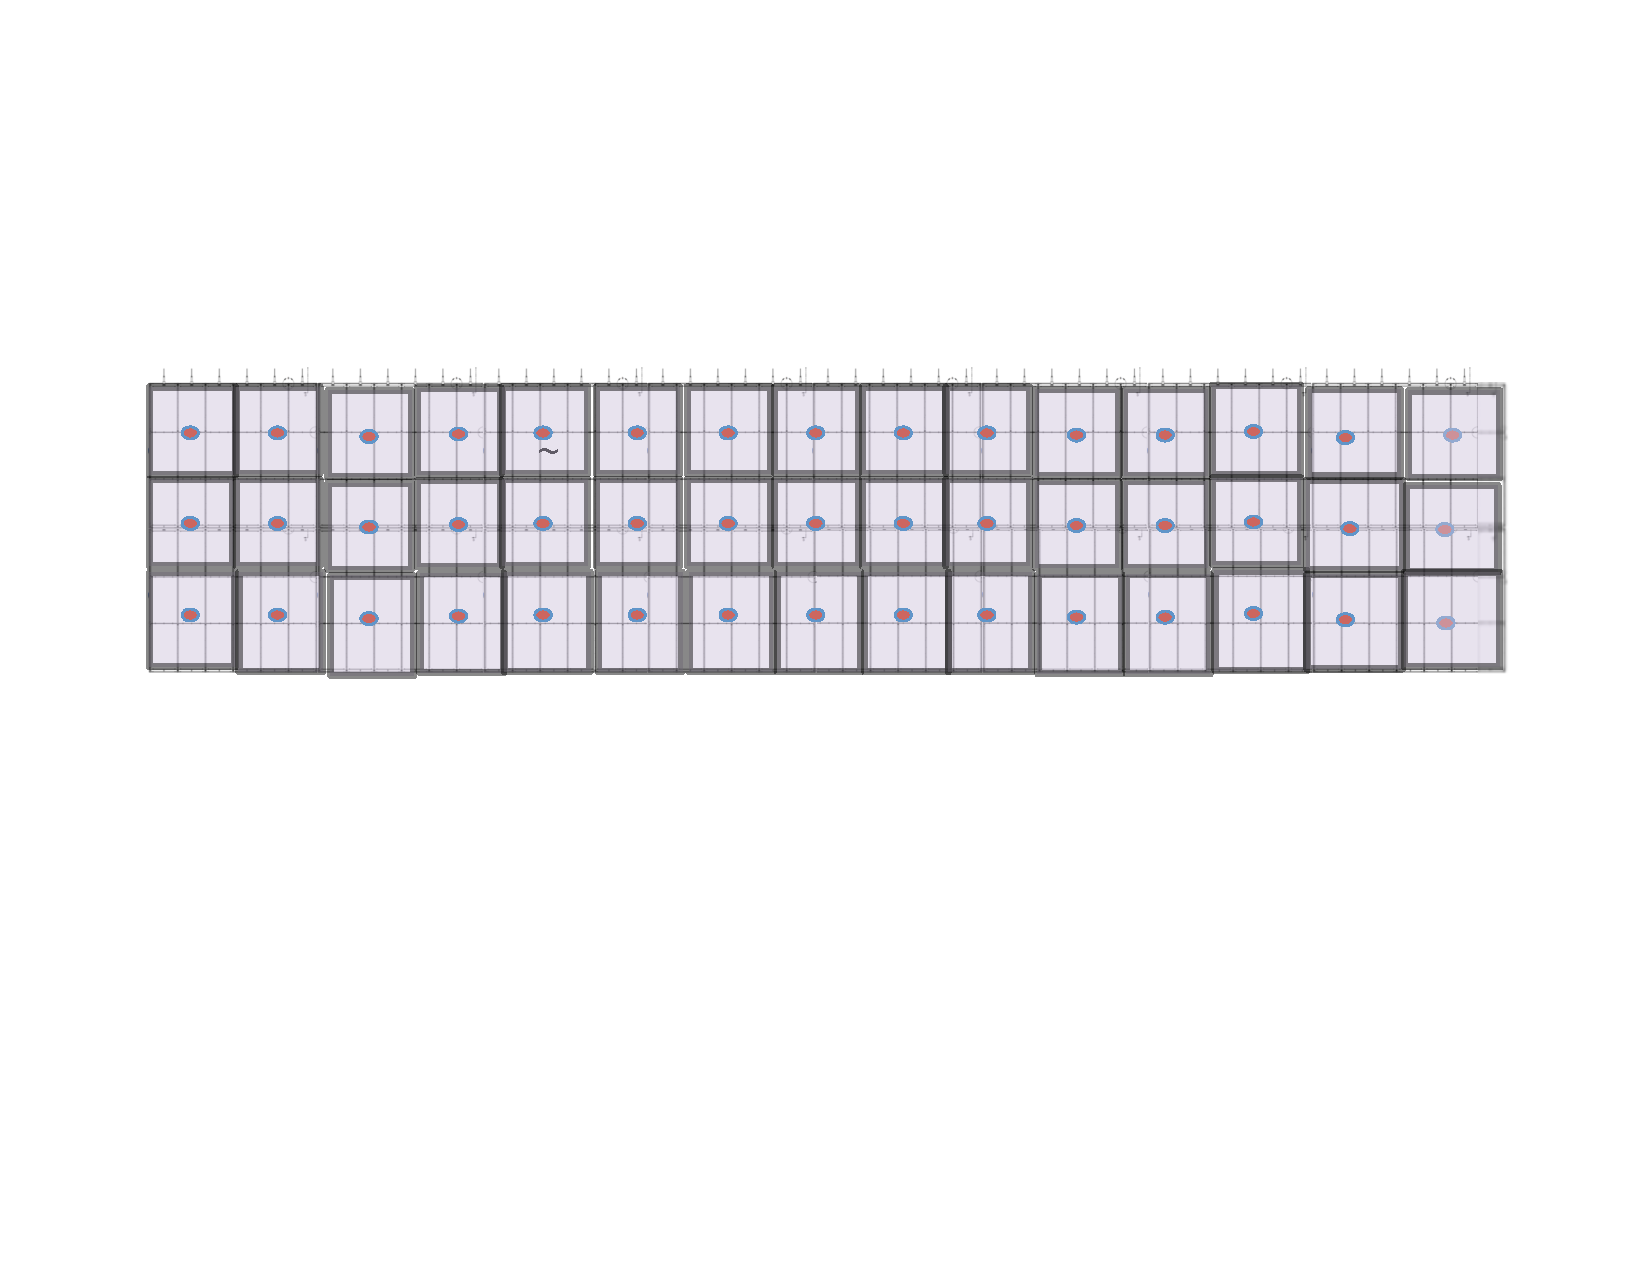
\includegraphics[angle=0,width=0.9\textwidth]{graphics/pds-calibration-cpa}
\end{dunefigure}

Quartz fibers, \SIrange{10}{30}{m} long, are used to transport light from the optical feedthrough (at the cryostat top) through the \dword{fc} \dword{gp}, and through \dword{fc} strips to the \dword{cpa} top frame. 
These fibers are then optically connected to diffusers located on the \dword{cpa} panels using fibers that are \SIrange{2}{10}{m} long. 
The diffusers, \SI{2.5}{cm} in diameter, are mounted on the cathode plane panels acting as light sources to illuminate \dwords{pd} embedded in the \dword{apa}s. There will be \num{45} diffusers uniformly distributed across each of the \dword{spmod} cathode planes facing \dword{apa}s, as indicated in 
Figure~\ref{fig:pds-calmon-cpa-diffusers}. Each diffuser will illuminate an area of approximately $\SI{4}{m}\times\SI{4}{m}$ on the \dword{apa}s that are \SI{3.6}{m} away. 

The diffusers reside at the \dword{cpa} potential, so the \dword{hv} system places a requirement on the fiber electrical resistance to protect the cathode from experiencing electrical breakdown along this path. This requirement is easily met by the fibers. 

As demonstrated in \dword{pdsp}, the system performs the required calibration and monitoring tasks with minimal impact on the \dshort{tpc} design and function. 
